\chapter{Attention Mechanism}
\section{Introduction}
In this section, we will focus on the deep learning models, the first one being a bidirectional LSTM and the second one an attention layer is added to this LSTM. But it is need to use another text embedding in order to work with LSTM. Indeed, tf-idf create a sparse matrix with each row corresponding to a value for a given word. This means that the order of the words are lost. In order to solve this, word2vec\cite{Mikolov2013} is used. It allows matching words to continuous vectors of a given size with interesting properties. Another method, which consists in making word embedding as tuning parameters will be used.
\section{Text to Vectors}
\subsection{Word2Vec}
Word2Vec comes in two fashions: continuous bag of words (CBOW) and skip gram. It is originally designed to predict a word given a context. For instance, given two previous words and the next two words, which word is the most likely to take place between them. But it appears that the hidden representation of these words works well as word embedding and has very interesting properties such that words with similar meaning have similar vector representation. It is also possible to perform arithmetic that captures information such as singular, plural or even capital and countries. For example, we have that $dog - dogs \approx cat - cats$ but also $Paris - France \approx Berlin - Germany$. \\

It is possible to visualize these relationships by using t-SNE for projecting high dimensions word vectors in 2D space. The results of various relationships can be seen at \textbf{Figure \ref{fig:chap4:word2vec}}.
\begin{figure*}
 \centering
 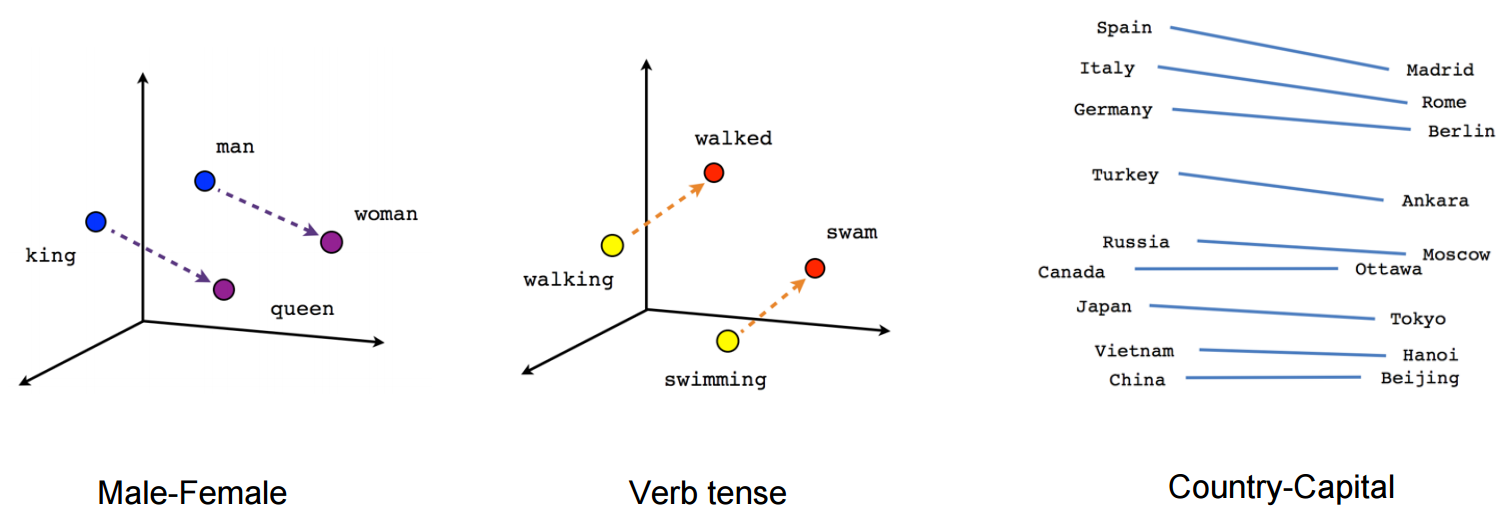
\includegraphics[width=\textwidth]{images/chapitre4/linear-relationships}
 \caption{Relationships between different words with t-SNE dimensionality reduction. }
 \label{fig:chap4:word2vec}
\end{figure*}
\subsubsection{How does it work?} 
As the original authors did not intend this kind of result, Xin Rong\cite{Rong2014} did a good job explaining how it works. 
Let V be the size of the vocabulary and that there is only one word in the CBOW model, it give \textbf{Figure \ref{fig:chap4:CBOW}} models. 
\begin{figure*}
 \centering
 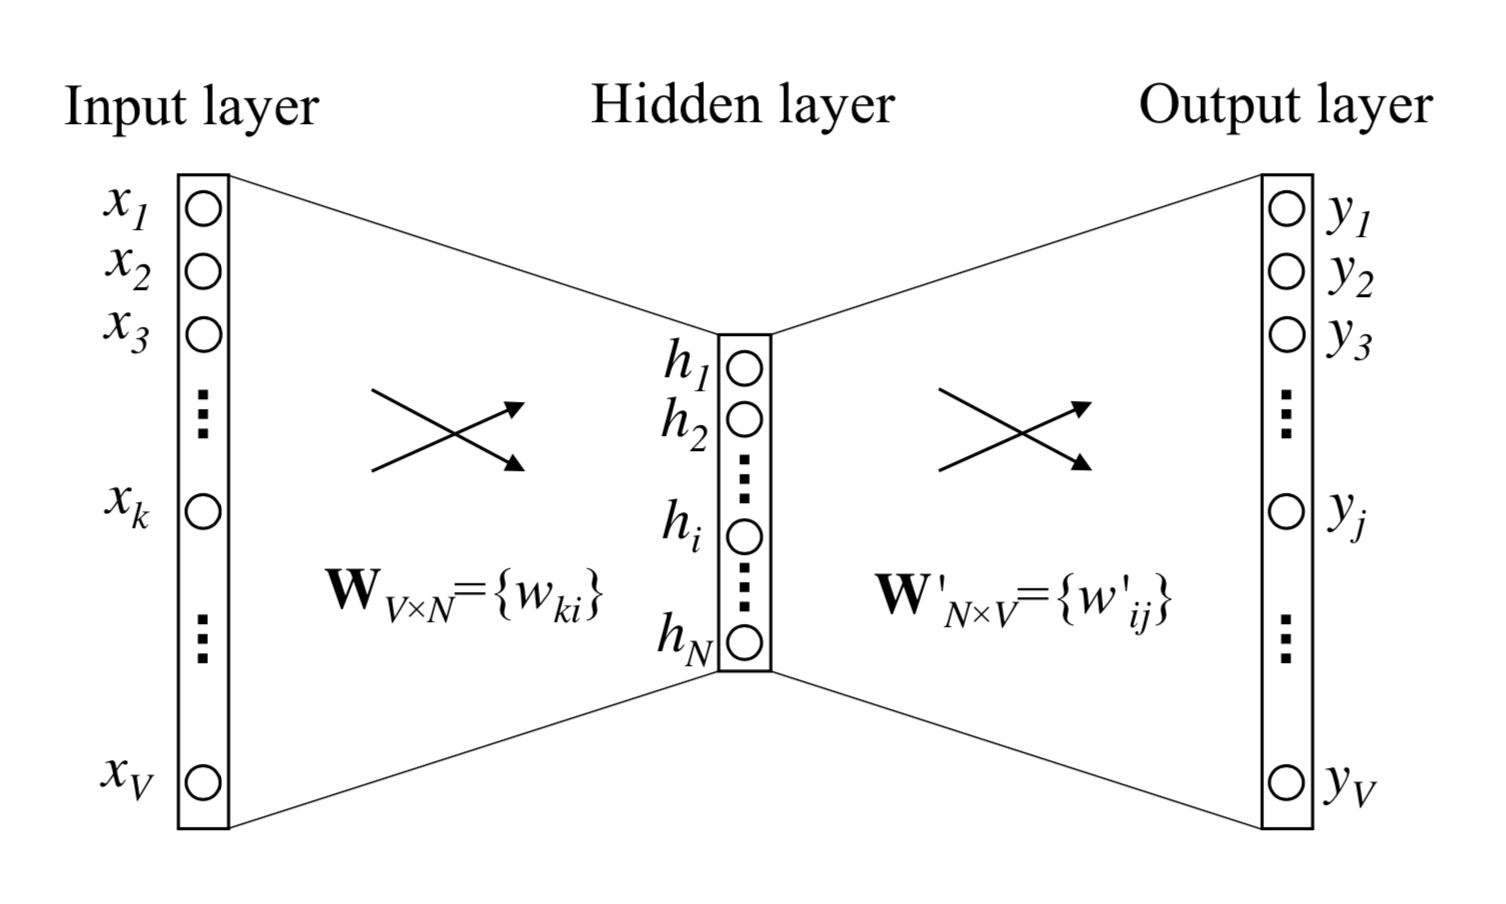
\includegraphics[width=\textwidth]{images/chapitre4/CBOW}
 \caption{A simple CBOW model with only one word in the context}
 \label{fig:chap4:CBOW}
\end{figure*}
Each word is encoded as a one-hot vector of size V. That means that it is a sparse vector full of zeros except for the position assigned to that word which is one. The hidden layer is computed as 
\begin{equation}
 \mathbf{h} = \mathbf{W^Tx}
\end{equation}
Where $\mathbf{W^{V \times N}}$ is the weight matrix to optimize over. 
The output layer values are computed as 
\begin{equation}
 \mathbf{Y} = \mathbf{W'^Th}
\end{equation}
As before $\mathbf{W'^{N \times V}}$ is also a weight matrix to optimize. The loss can be computed as softmax cross entropy. \\

It is also possible to make the opposite: predicting the context given a single input word. This is the skip-gram model. In this case the loss becomes \textbf{Equation \ref{eq:loss}}.
\begin{equation}
 E = - \sum_{c=1}^C u_{j^*_c} + C \cdot \sum_{j' = 1}^V \exp(u_{j'}) \ \label{eq:loss}
\end{equation}
$j_c^*$ is the index of the cth output context word and $u_{j^*_c}$ is the score of the jth word in the vocabulary for the cth context word. Finally, the embedding that is used are the value of the hidden layers produced for a given word. 
\begin{figure*}
 \centering
 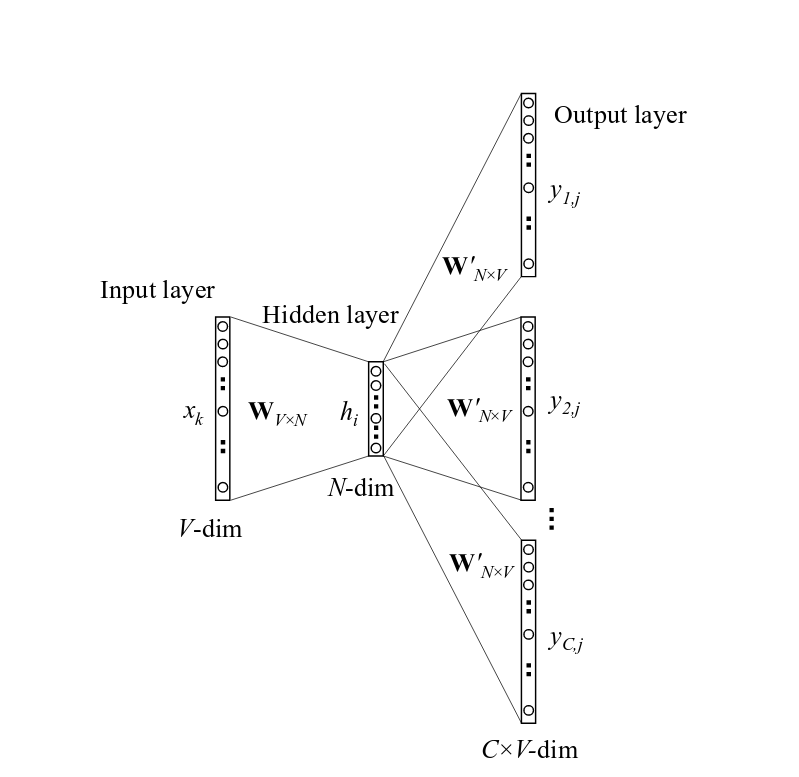
\includegraphics[width=\textwidth]{images/chapitre4/skip-gram}
 \caption{Skip-gram model with multiple outputs.}
 \label{fig:chap4:skip-gram}
\end{figure*}
\section{LSTM}
LSTM or Long Short Term Memory\cite{Hochreiter1997LongSM} is a kind of recurrent neural network that fits well to temporal or sequential input such as texts. A RNN is a type of neural network where the hidden state is fed in a loop with the sequential inputs. There are usually shown as unrolled version of it (\textbf{Figure \ref{fig:chap4:RNN_unroll}}). Each of the $X_i$ being one value in the sequence.\\

In this case, $X_i$ values are word vectors. There are two possibilities, either use pre-trained vector with word2vec or make $X_i$ inputs a parameter to learn in the same way as it works for the Word2Vec algorithm, having a one-hot encoding of the word and a matrix of weights to tune. Each method will be used. \\

Recurrent Neural Networks do not works very well with long-term dependencies, that is why LSTM have been introduced. It is made of an input gate, an output gate and a forget gate that are combined in \textbf{Equation \ref{eq:LSTM}}.
\begin{figure}
 \centering
 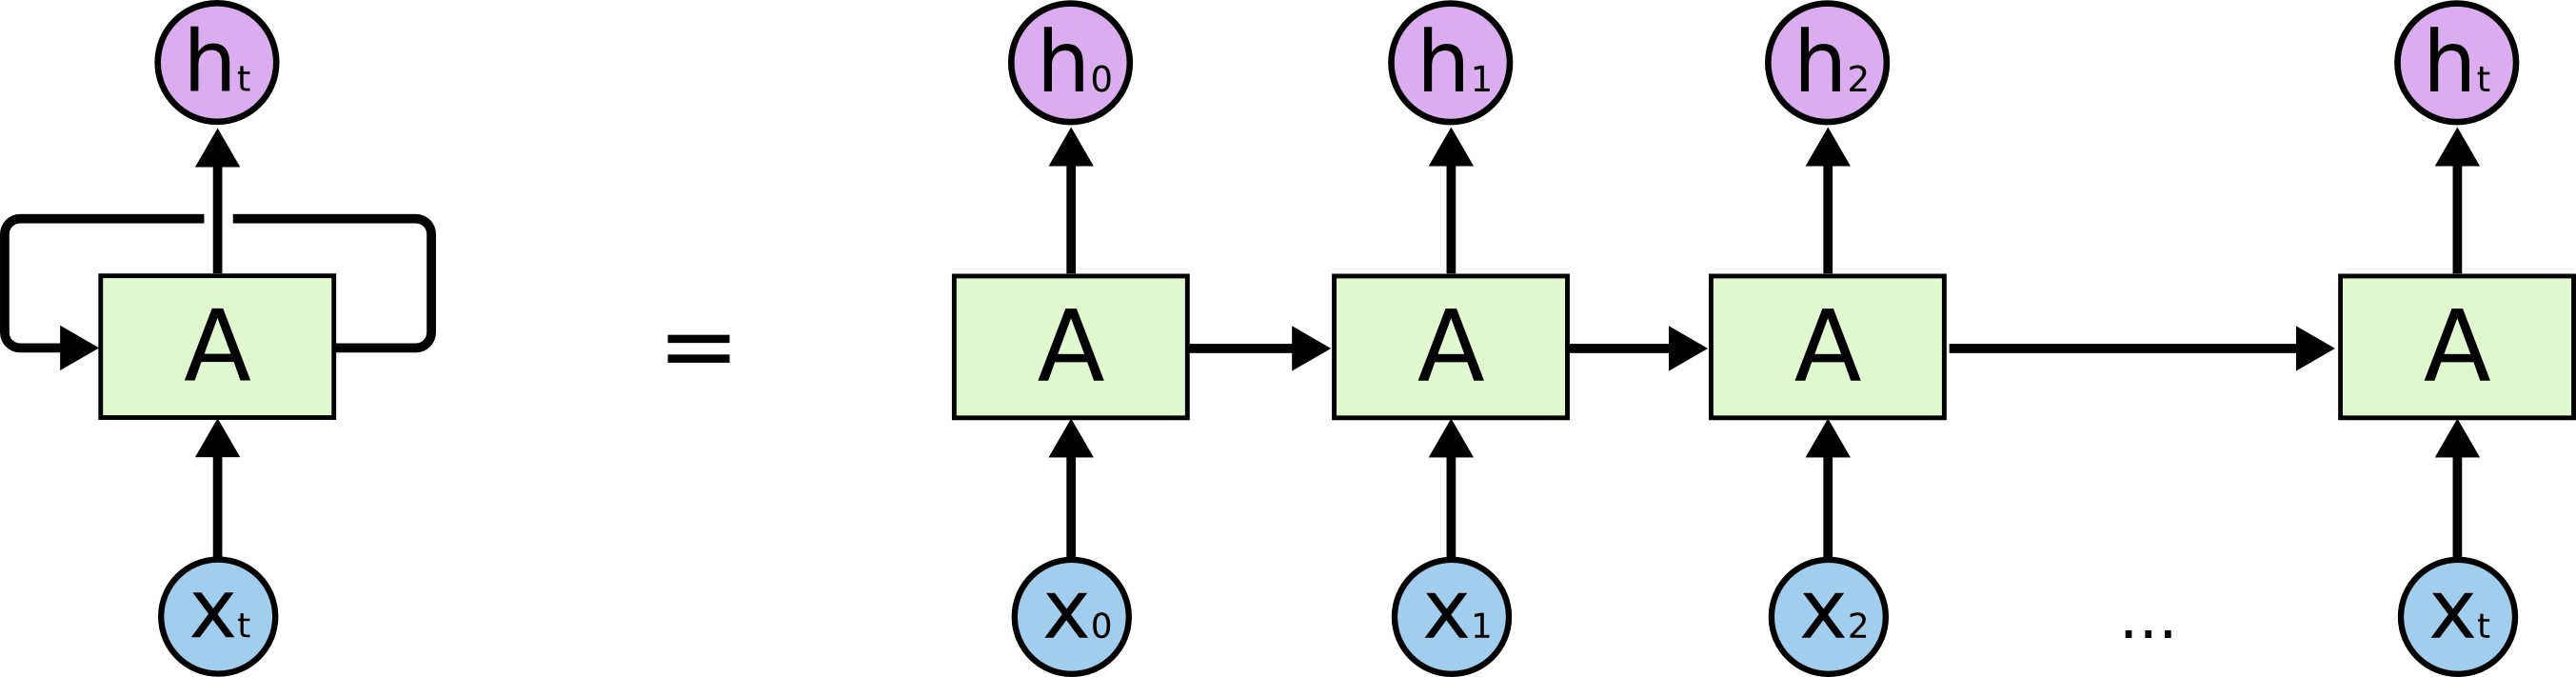
\includegraphics[width=\textwidth]{images/chapitre4/RNN-unrolled.png}
 \caption{Unrolled RNN (Understanding LSTM Networks, \url{https://colah.github.io/posts/2015-08-Understanding-LSTMs/)}}
 \label{fig:chap4:RNN_unroll}
\end{figure} 
\begin{align} \label{eq:LSTM}
 f_t &= \sigma_g(\mathbf{W}_f x_t + \mathbf{U}_fh_{t-1} + b_f)\\
 i_t &= \sigma_g(\mathbf{W}_i x_t + \mathbf{U}_ih_{t-1} + b_i)\\
 o_t &= \sigma_g(\mathbf{W}_o x_t + \mathbf{U}_oh_{t-1} + b_o)\\
 c_t &= f_t \circ c_{t-1} + i_t \circ \sigma_c(\mathbf{W}_cx_t + \mathbf{U}_c h_{t-1} + b_c)\\
 h_t &= o_t \circ \sigma_h (c_t)
\end{align}
\textbf{Figure \ref{fig:chap4:LSTM-gates}} shows how it works.
\begin{figure}
 \centering
 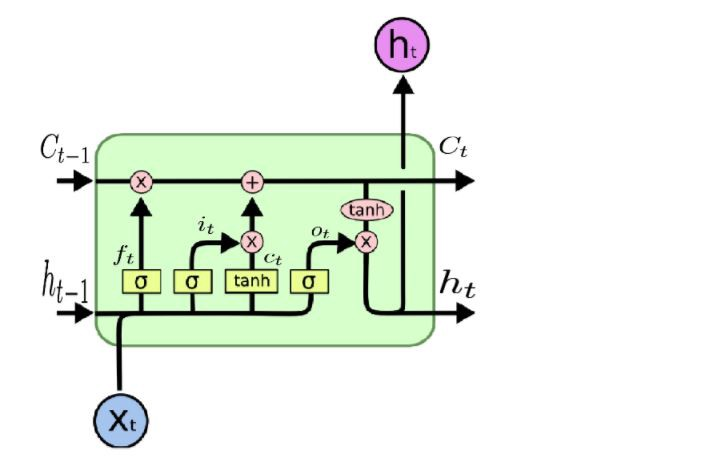
\includegraphics[width=0.6\textwidth]{images/chapitre4/LSTM1.jpeg}
 \caption{LSTM gates, \\ \url{https://hackernoon.com/understanding-architecture-of-lstm-cell-from-scratch-with-code-8da40f0b71f4)}}
 \label{fig:chap4:LSTM-gates}
\end{figure} 
A bidirectional LSTM works the same way, but the input is fed in the two directions, from the start to the end and from the end to the start.
\section{Attention Mechanism}
Attention mechanism\cite{zhou-etal-2016-attention,Vaswani2017AttentionIA} adds an extra layer between LSTM outputs and the final output of the network. It merges word-level features into sentence features using a weight vector. \\

\begin{figure}
 \centering
 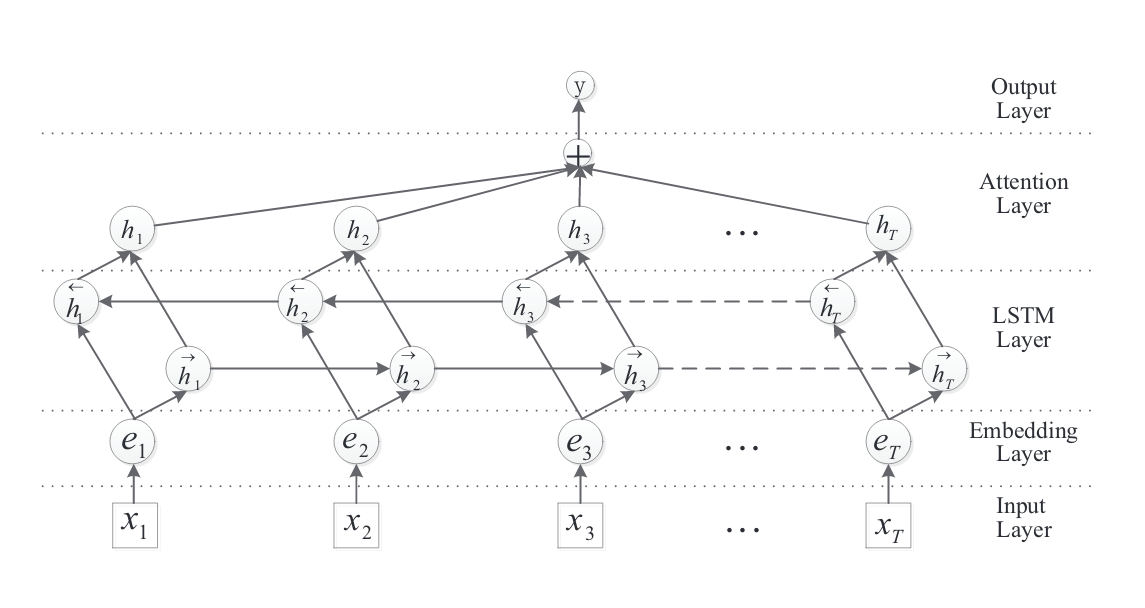
\includegraphics[width=\textwidth]{images/chapitre4/attention.png}
 \caption{Bidirectional LSTM Model With Attention}
 \label{fig:chap4:attention}
\end{figure}
Outputs sequence of the LSTM is summed element-wise in order to merge them. We have that $h_i = [\overrightarrow{h_i} + \overleftarrow{h_i}]$, $\overrightarrow{h_i}$ and $\overleftarrow{h_i}$ begin the outputs i of sequence in each direction as show at \textbf{Figure \ref{fig:chap4:attention}}.\\
Let’s $H$ be a matrix of the concatenation of all the $h_i$, 
\begin{equation}
 H = [h_1,h_2,...,h_T]
\end{equation}
Where T is the sequence length. 
Then we define 
\begin{align}
 M &= \tanh(H)\\
 \alpha &= softmax(w^TM) \\
 r &= H \alpha^T 
\end{align}
Finally, we compute $h^* = \tanh(r)$.
For the classification, it uses a softmax classifier as $\hat{p}(y|S) = softmax(W^Sh^* + b)$. Originally the loss function is the negative log likelihood, but as in this case it is a binary classification I used binary cross entropy. 
\section{Results}
\subsection{Methodology}
In order to train the models and perform hyper parameters optimization grid search have been used when it was possible (on the liar-liar dataset) and knwoleadge acquired there have been used in order to tune parameters for the networks on the \textbf{Fake News Corpus}. In addition, in order to find the best parameters among all tested with gird search, for each metric, the training epochs having the highest validation value for those metrics have been chosen. \\

All the models have been trained using adam optimizer and initialized using a normal distribution for the weights. \\

As SMOTE cannot be used on the \textbf{Fake News Corpus} dues to the size of the corpus, in order to rebalance the dataset the minority class have been over sampled by feeding multiple times the same input by looping through them. 
\subsection{Liar-Liar dataset results}
As explained earlier, both models have been trained using different embedding: the first one being pre-trained word2vec vectors of size 300 and the second one being a tunable parameter with different embedding size.
\subsubsection{LSTM}
When it comes to LSTM trained on liar-liar dataset, it simply does not works. It classifies almost all the texts as being from the same class. Although, it reaches a good score on the training data, it does not manage to generalize correctly. \textbf{Figure \ref{fig:chap4:lstm2}} shows the recall, precision and f1-score and loss for training and testing set of the best models for the LSTM using word2vec. We can see that even if the training score increase, the testing values oscillate. \\

\begin{figure}
 \centering
 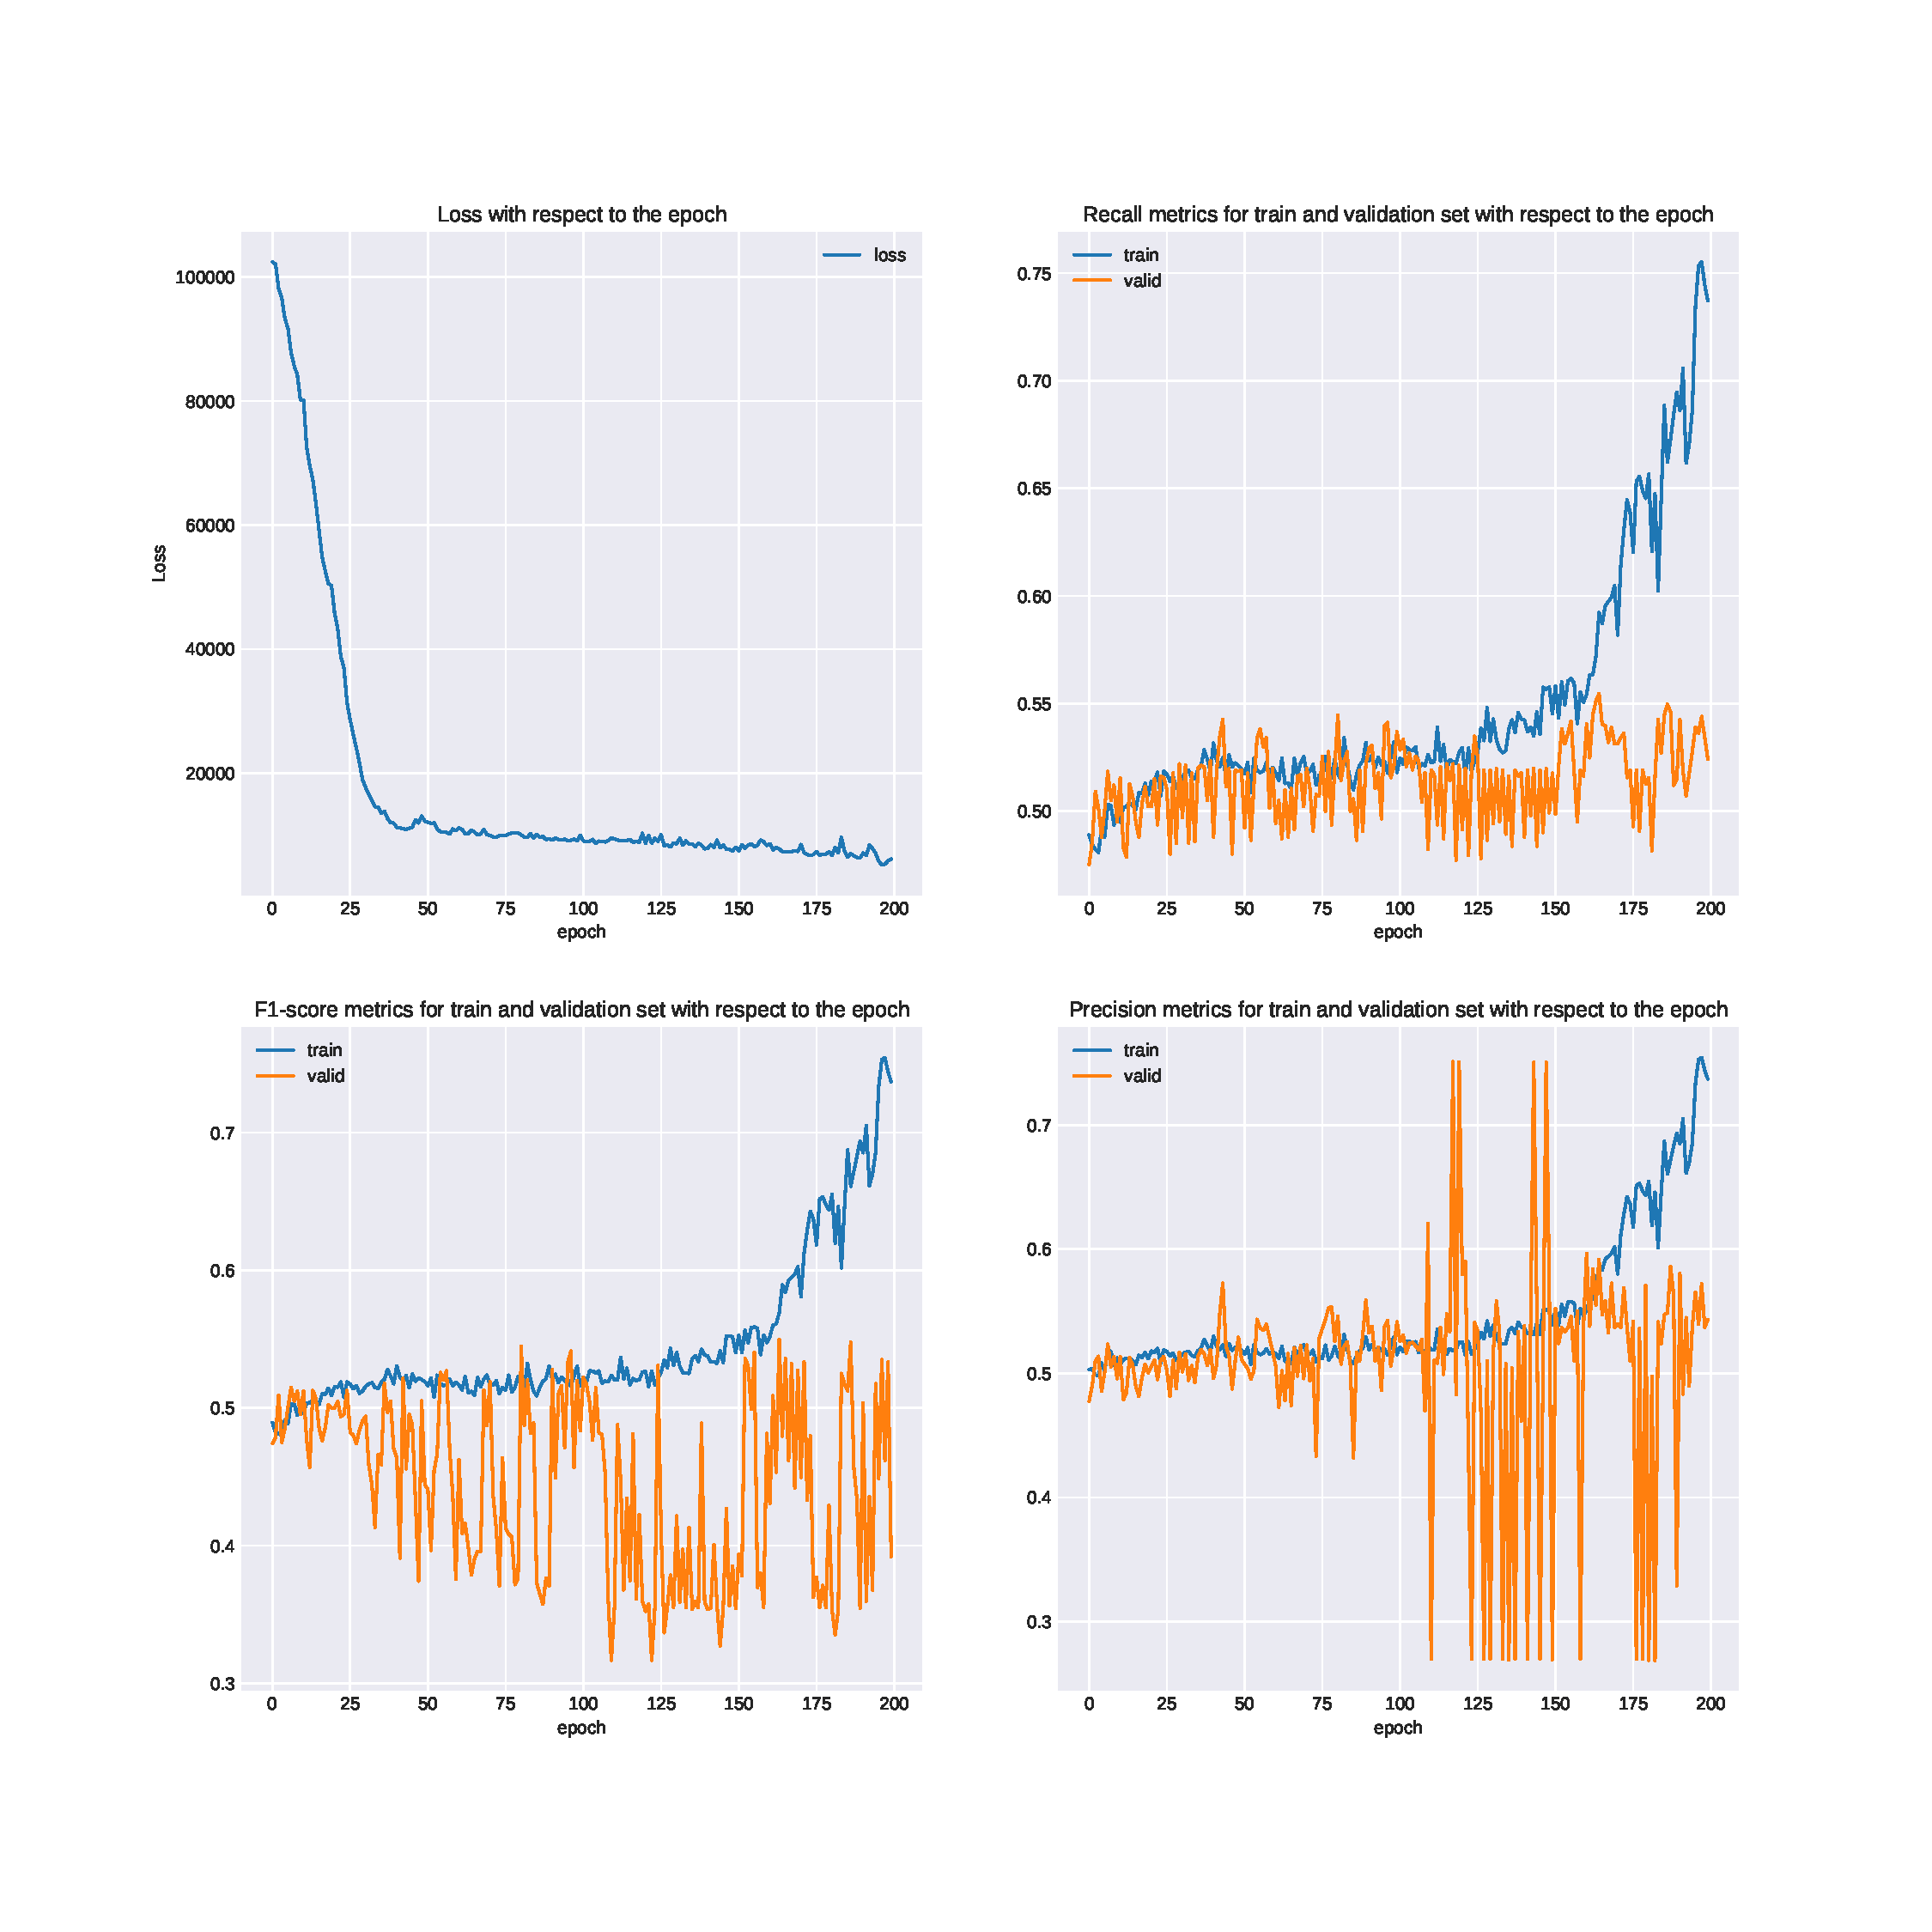
\includegraphics[width=\textwidth]{images/chapitre4/lstm2}
 \caption{Best LSTM With word2vec}
 \label{fig:chap4:lstm2}
\end{figure}
When training the models with word embedding as tunable parameters, the results slightly improve, with an average precision between $55\%$ and $60\%$. This can be seen at \textbf{Figure \ref{fig:chap4:lstm1}}. \\
The training was stopped after 200 iterations because the validation score was not improving anymore. 
\begin{figure}
 \centering
 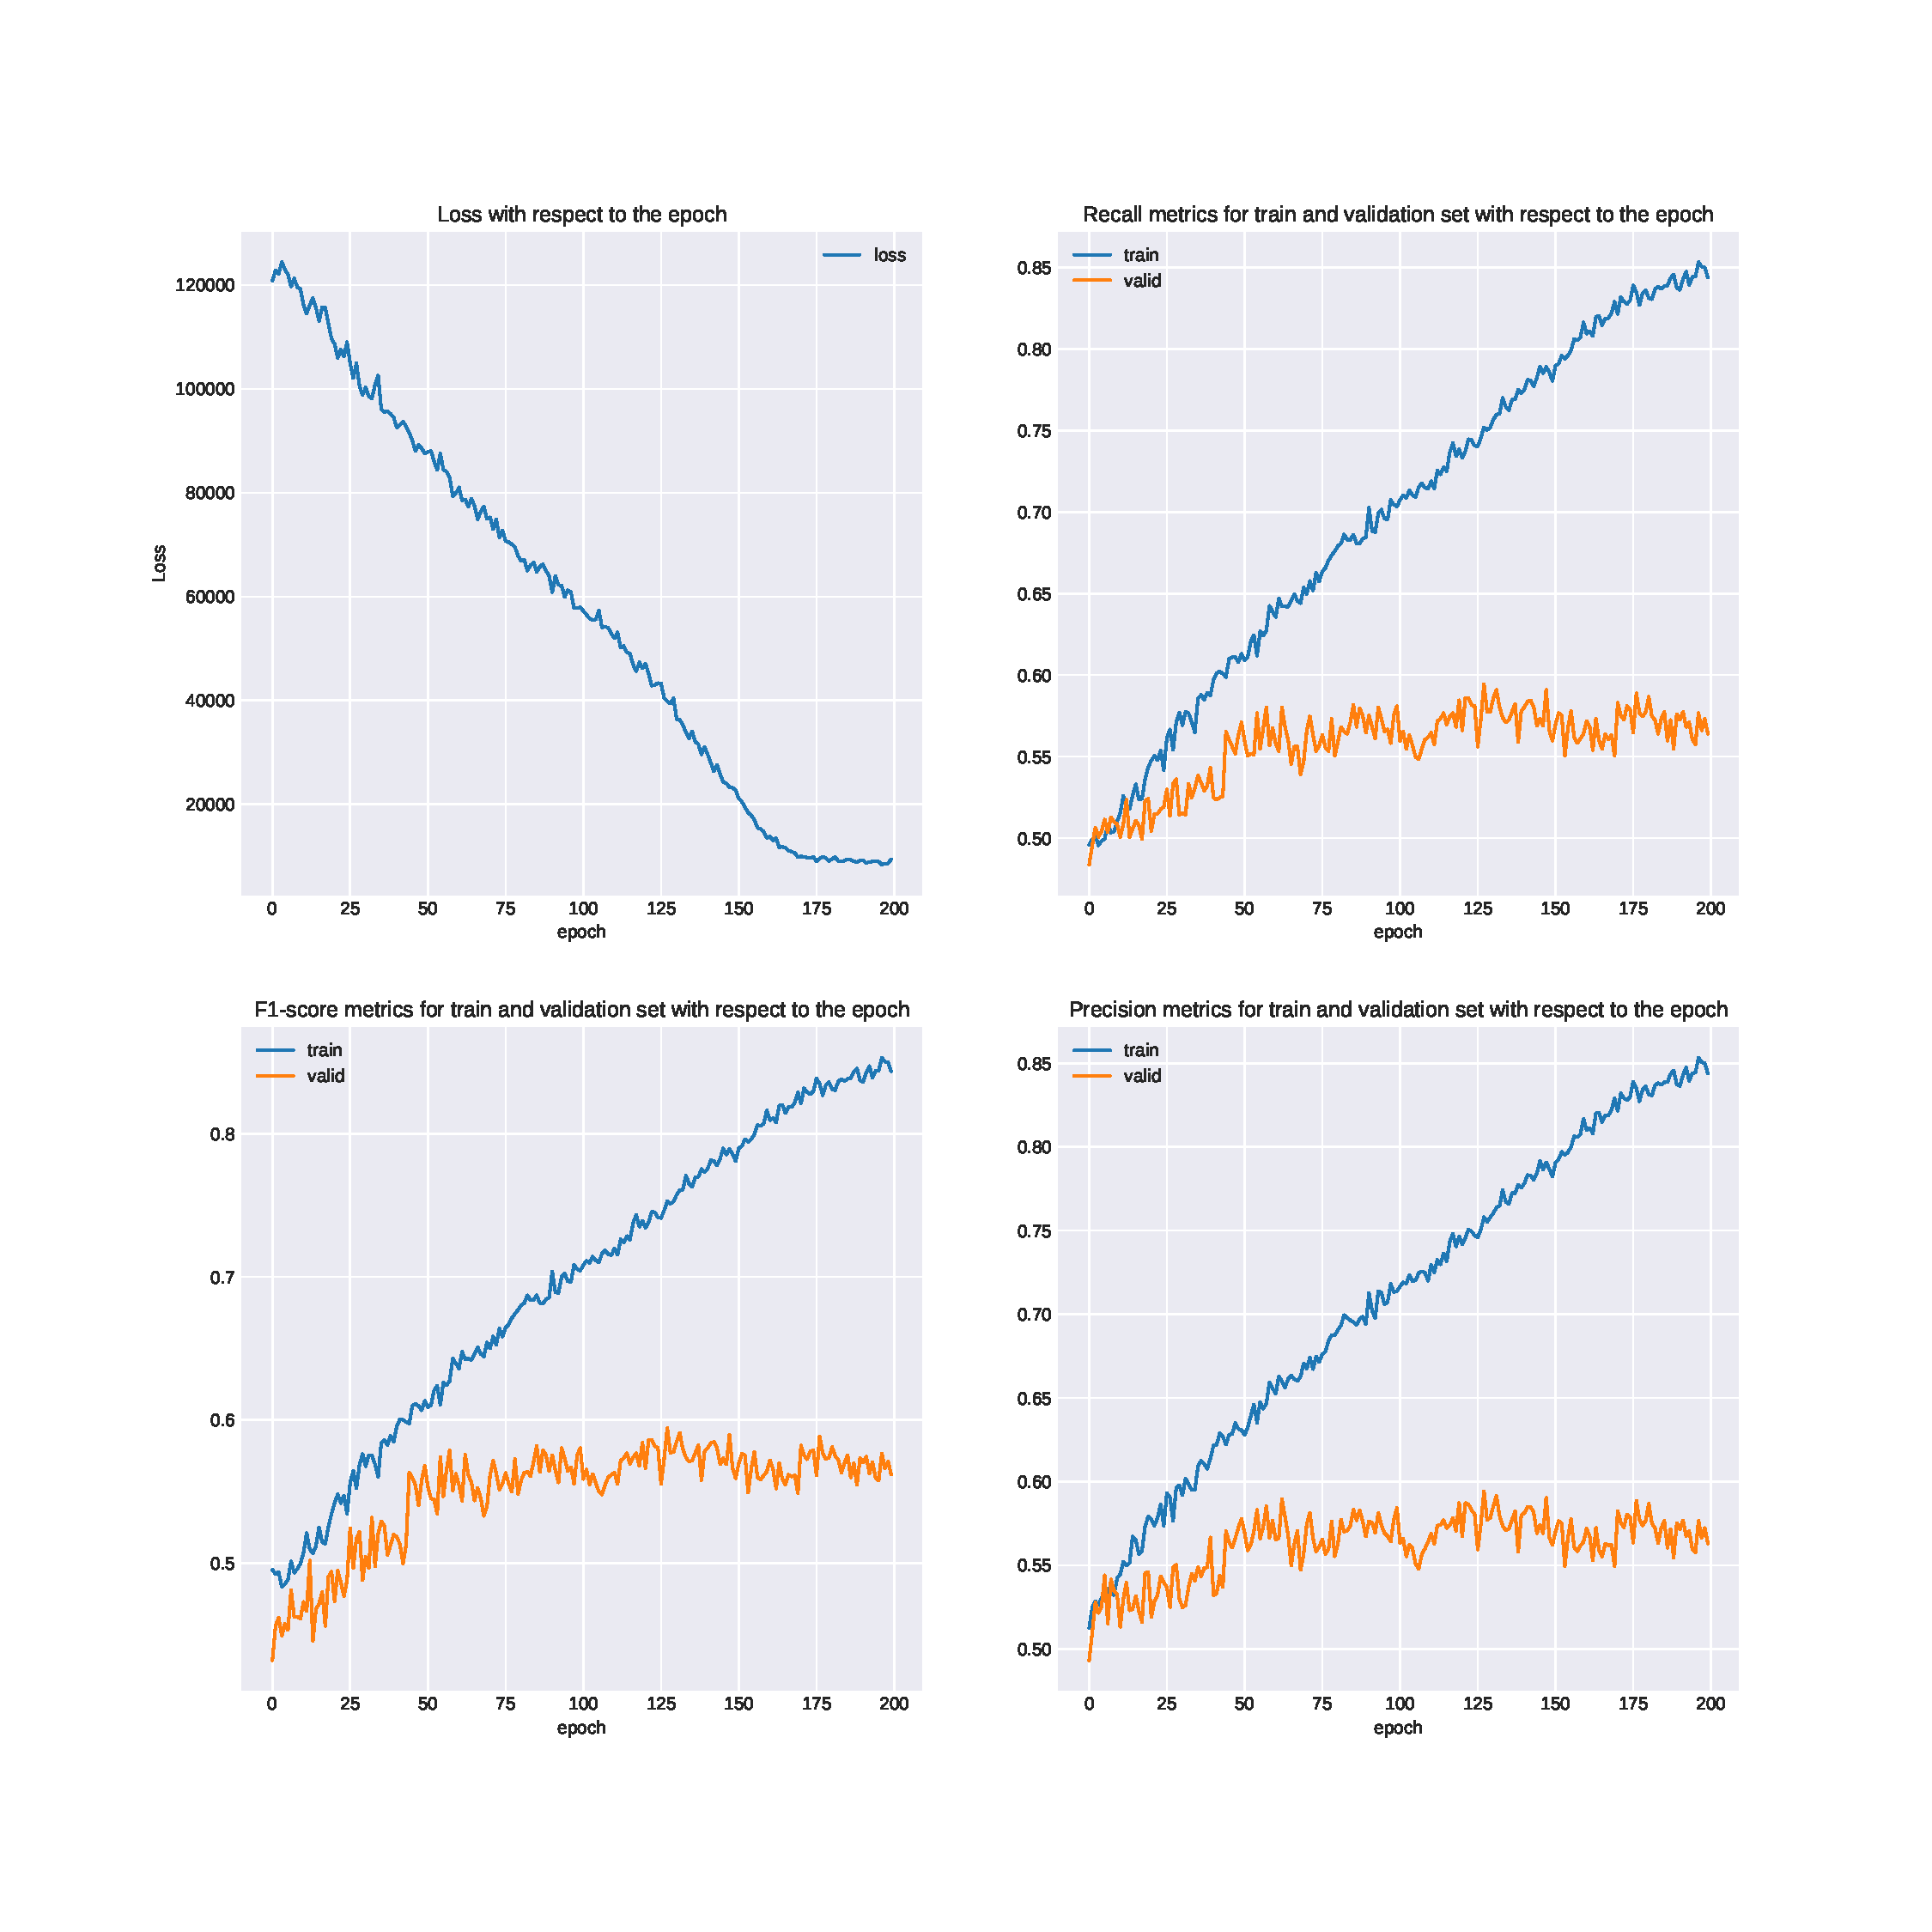
\includegraphics[width=\textwidth]{images/chapitre4/lstm1}
 \caption{Best LSTM with word embedding as tunable parameters.}
 \label{fig:chap4:lstm1}
\end{figure}

\subsection{Attention Mechanism}
We could think that adding an extra layer to such a bad model would not make any improvement and be useless, but adding an attention layer does improve a little the results. When using word2vec embedding, the best epoch reaches up to $62.9595\%$ of average accuracy, which is better than the simple LSTM. Because there are a lot of models with different parameters, it is interesting to look at the distribution of the results for the best epochs by fixing parameters one by one. \textbf{Figure \ref{fig:chap4:att1:confInt}} shows the $95\%$ confidence interval for precision for a fixed parameter. \\
\begin{figure}
 \centering
 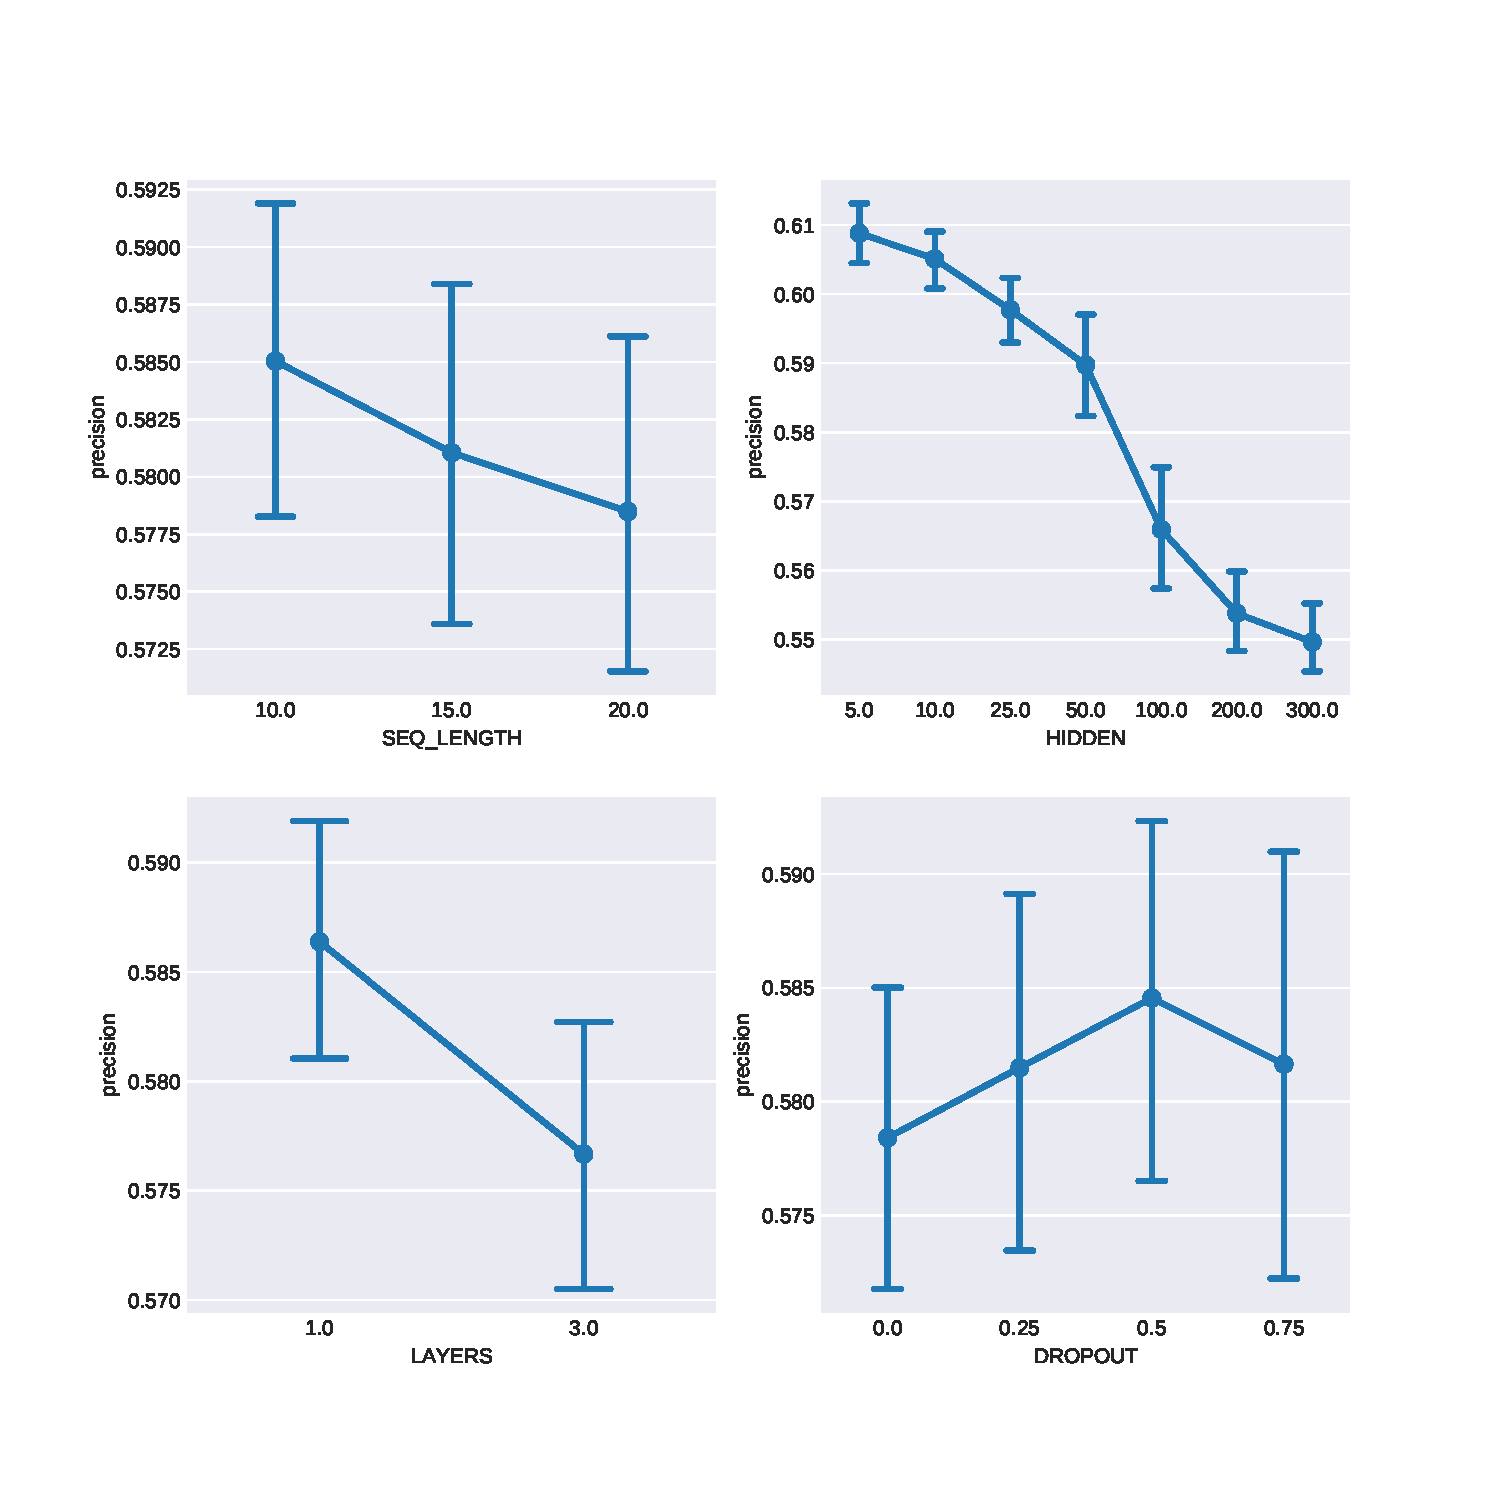
\includegraphics[width=\textwidth]{images/chapitre4/confInt_precision_liar_attention_word2vec}
 \caption{Confidence Interval of Precision for Each Parameter Value}
 \label{fig:chap4:att1:confInt}
\end{figure}
It shows that it is better to use fewer hidden units in the model, and only a single layer. The sequence length has a very small impact on the precision. Actually, the best model uses a sequence length of 20. \\\
The precision of the different models range from $53\%$ to $63\%$ (\textbf{Figure \ref{fig:chap4:att1:distPrecision}}.)
\begin{figure}
 \centering
 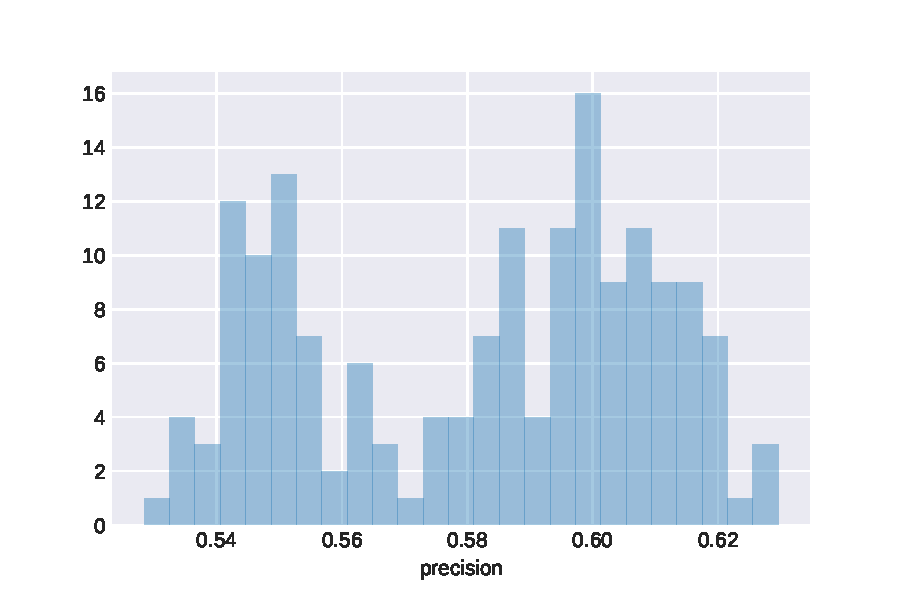
\includegraphics[width=\textwidth]{images/chapitre4/distplot_precision_liar_attention_word2vec}
 \caption{Distribution of the precision of best epochs for all the models trained with word2vec embedding.}
 \label{fig:chap4:att1:distPrecision}
\end{figure}
The training plot of the model that reaches the maximum precision can be seen at \textbf{figure \ref{fig:chap4:att1:train}}. It shows that after the 25th iteration, the validation values start to decrease, which is a sign of overfitting. \\

\begin{figure}
 \centering
 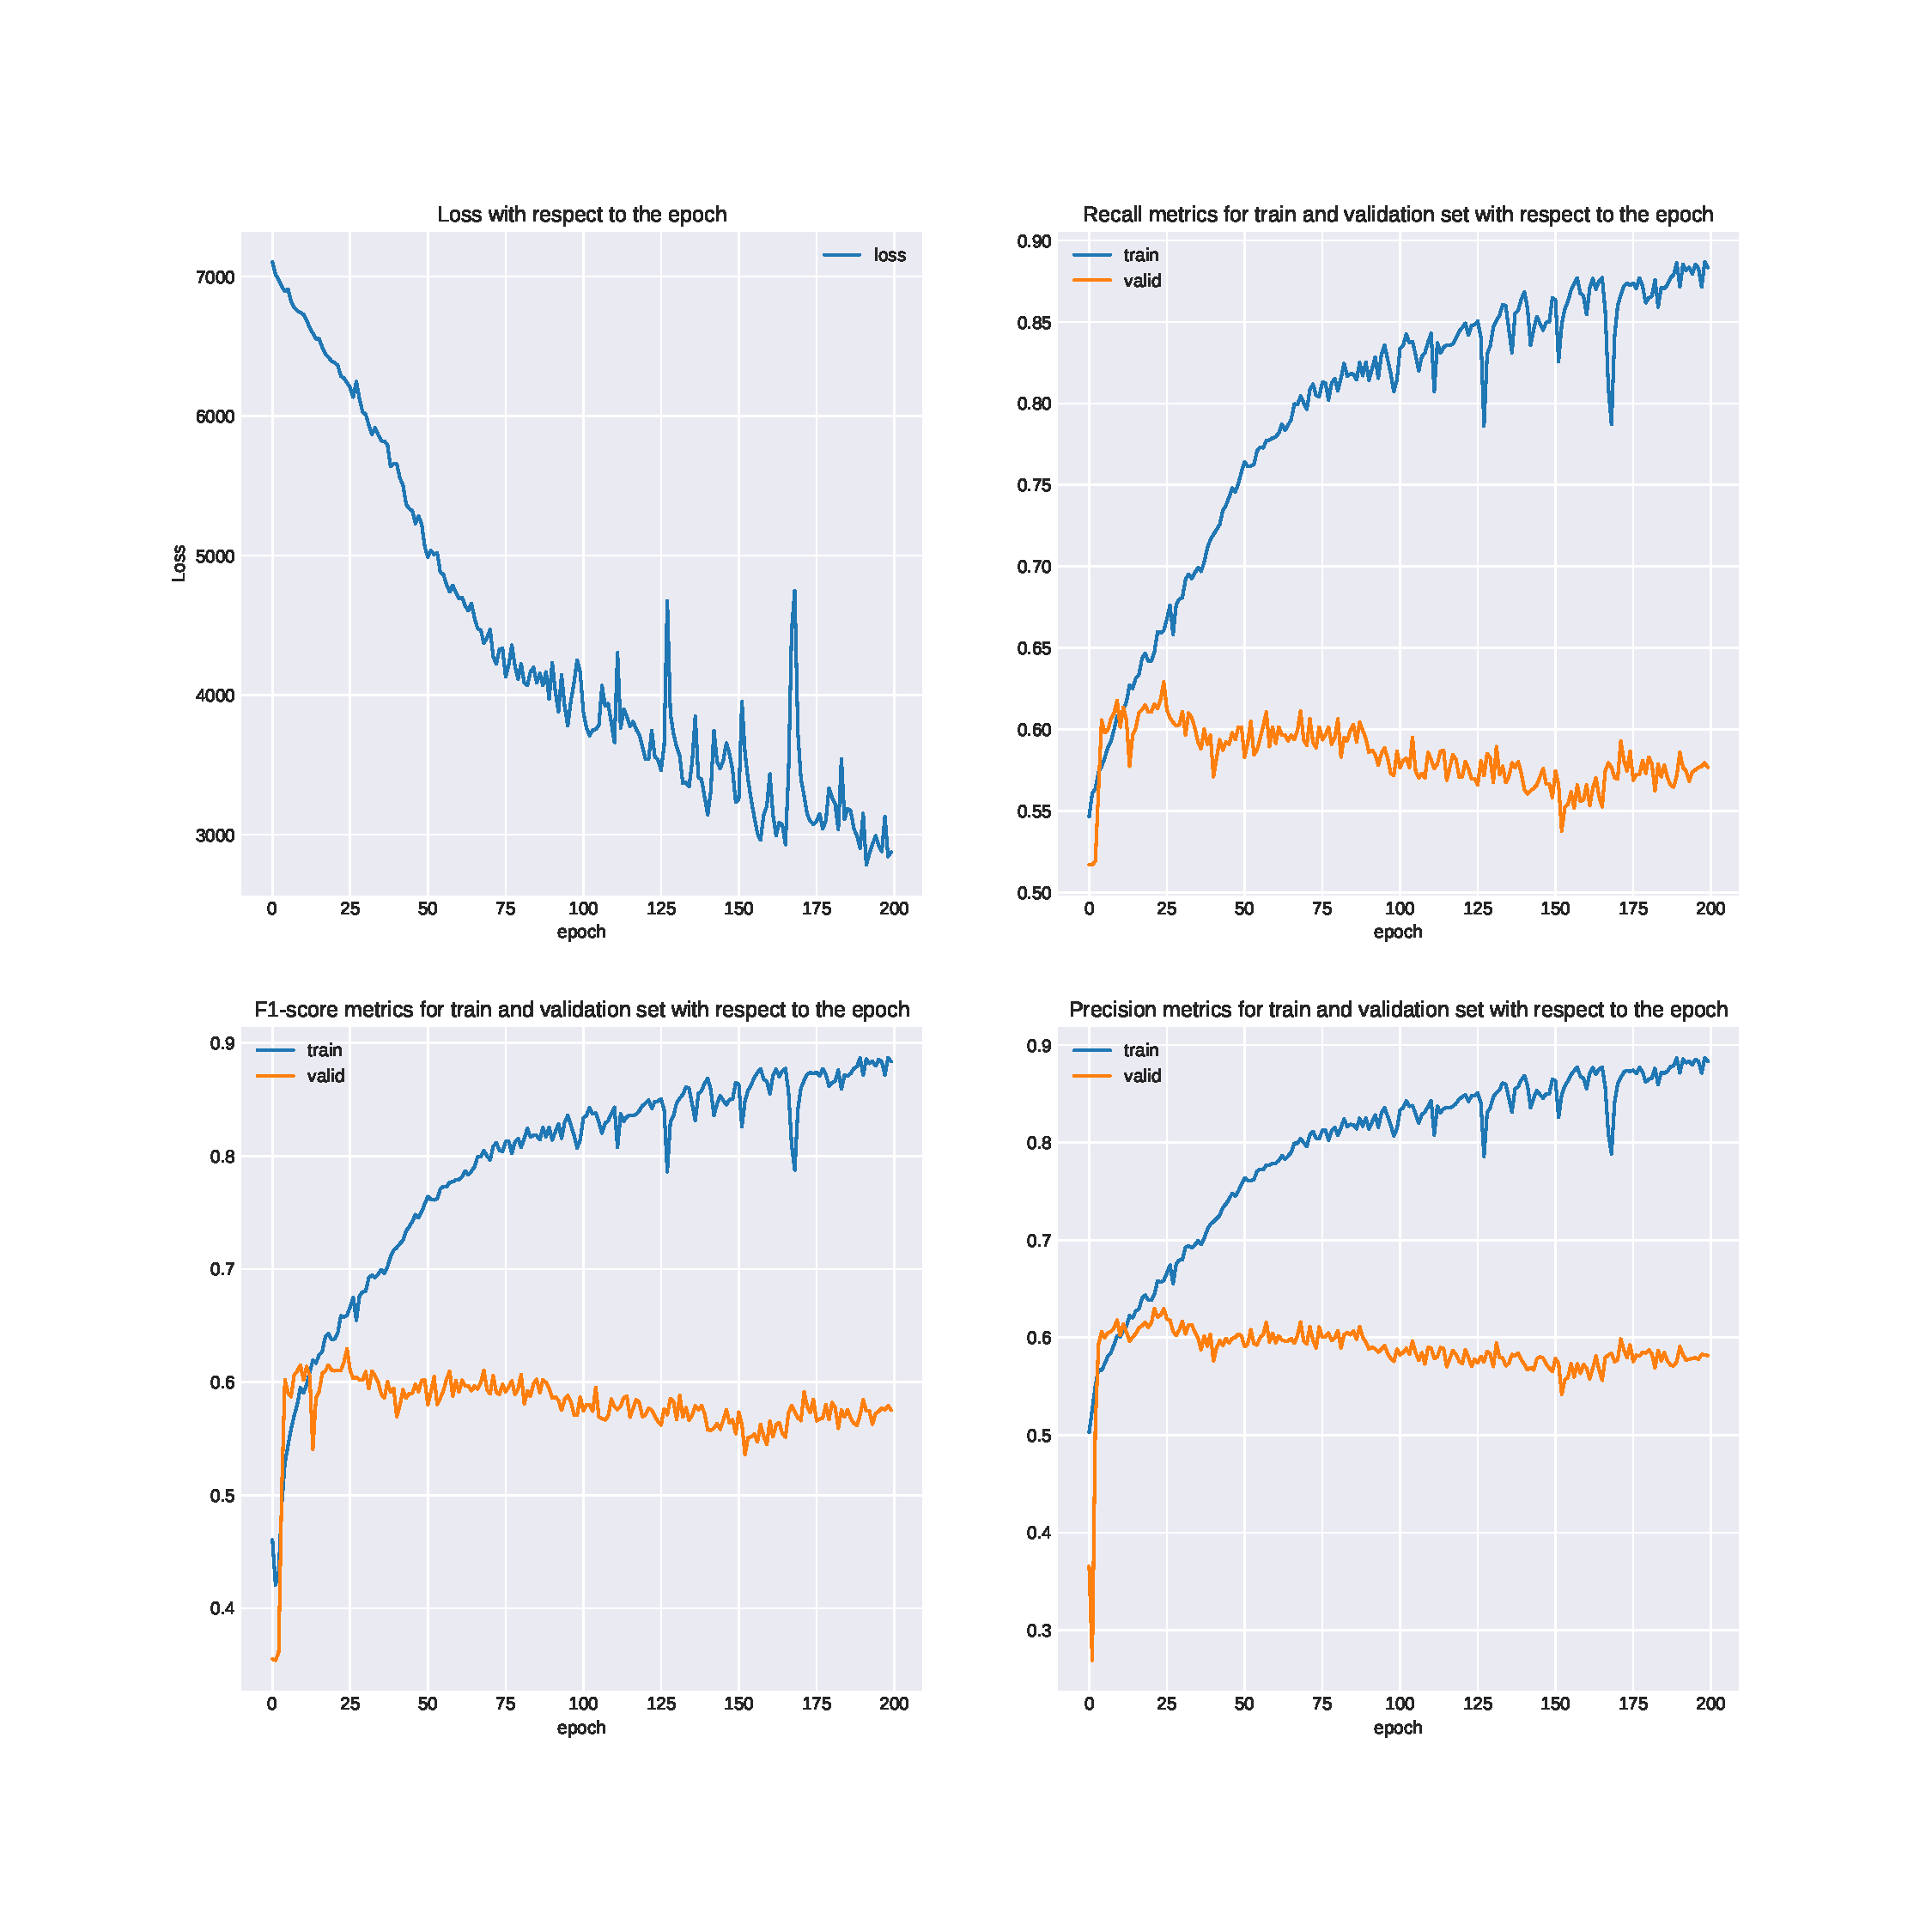
\includegraphics[width=\textwidth]{images/chapitre4/attention1}
 \caption{Training and validation of the model with top precision trained with word2vec embedding.}
 \label{fig:chap4:att1:train}
\end{figure}
Finally, there is the models where the embedding is a tunable parameter. The \textbf{Figure \ref{fig:chap4:att3:confInt2}} shows that in this case, the longer the sequence the better, and that as before using few hidden units perform better. In this case, variation has a wider range than when using word2vec. 
\begin{figure}
 \centering
 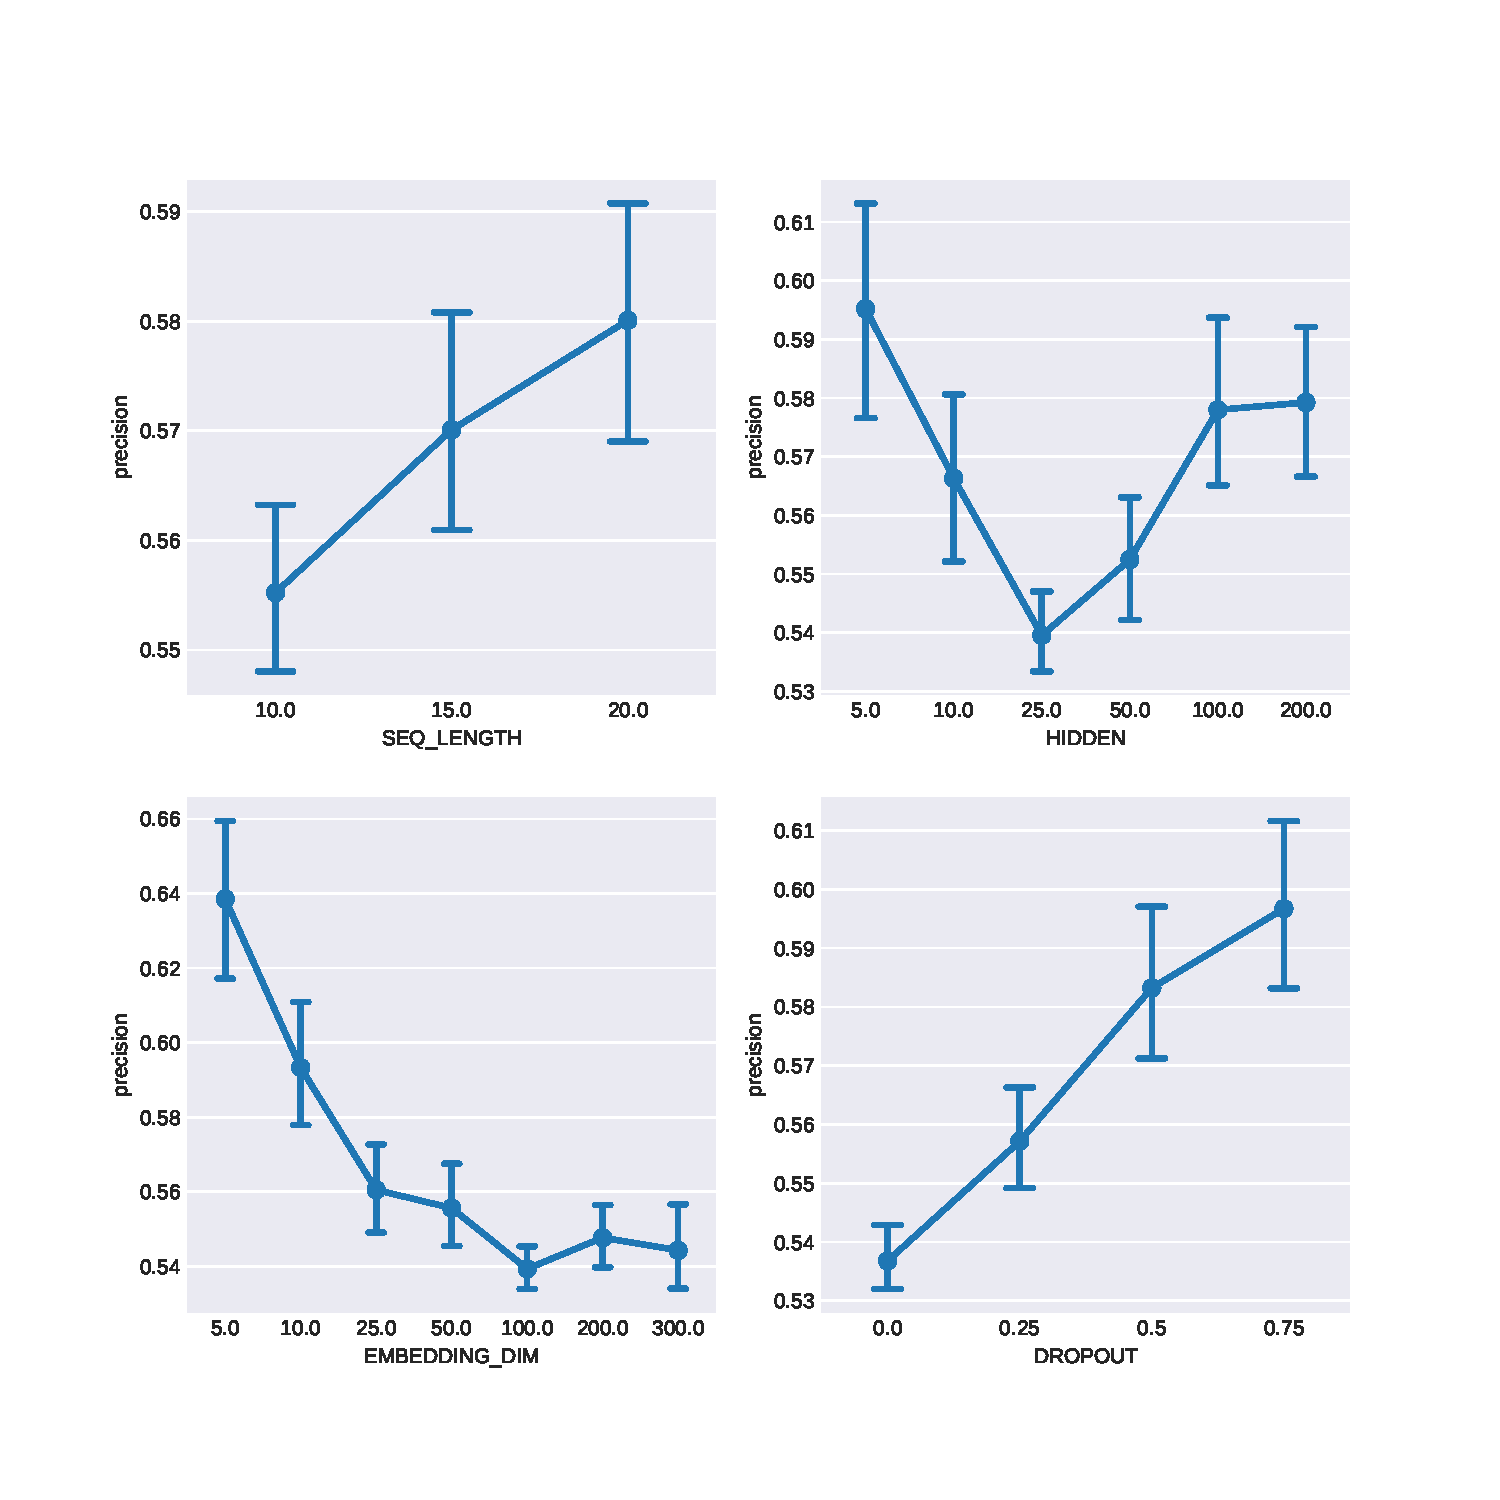
\includegraphics[width=\textwidth]{images/chapitre4/confInt_precision_liar_attention_200}
 \caption{Training and Validation of the Model With top Precision}
 \label{fig:chap4:att3:confInt2}
\end{figure}
There are a few models that have top precision higher than $75\%$, but looking at the training plot (\textbf{Appendix \ref{Appendix2}, Figure \ref{appendix2:training_plot1}}) shows that the model does not perform well. Because in particular case precision in not a good indicator of how well a model perform, f1-score will be used instead, as it is a balance between precision and recall. \\
And the best f1-score obtained is $0.55384$, which is quite smaller than the $0.63$ for the model using word2vec. The training plot is at \textbf{Figure \ref{fig:chap4:att3:f1}}. We can see that there is still room for improvement, the next step is to see what happens when training on more epochs. \\

\begin{figure}
 \centering
 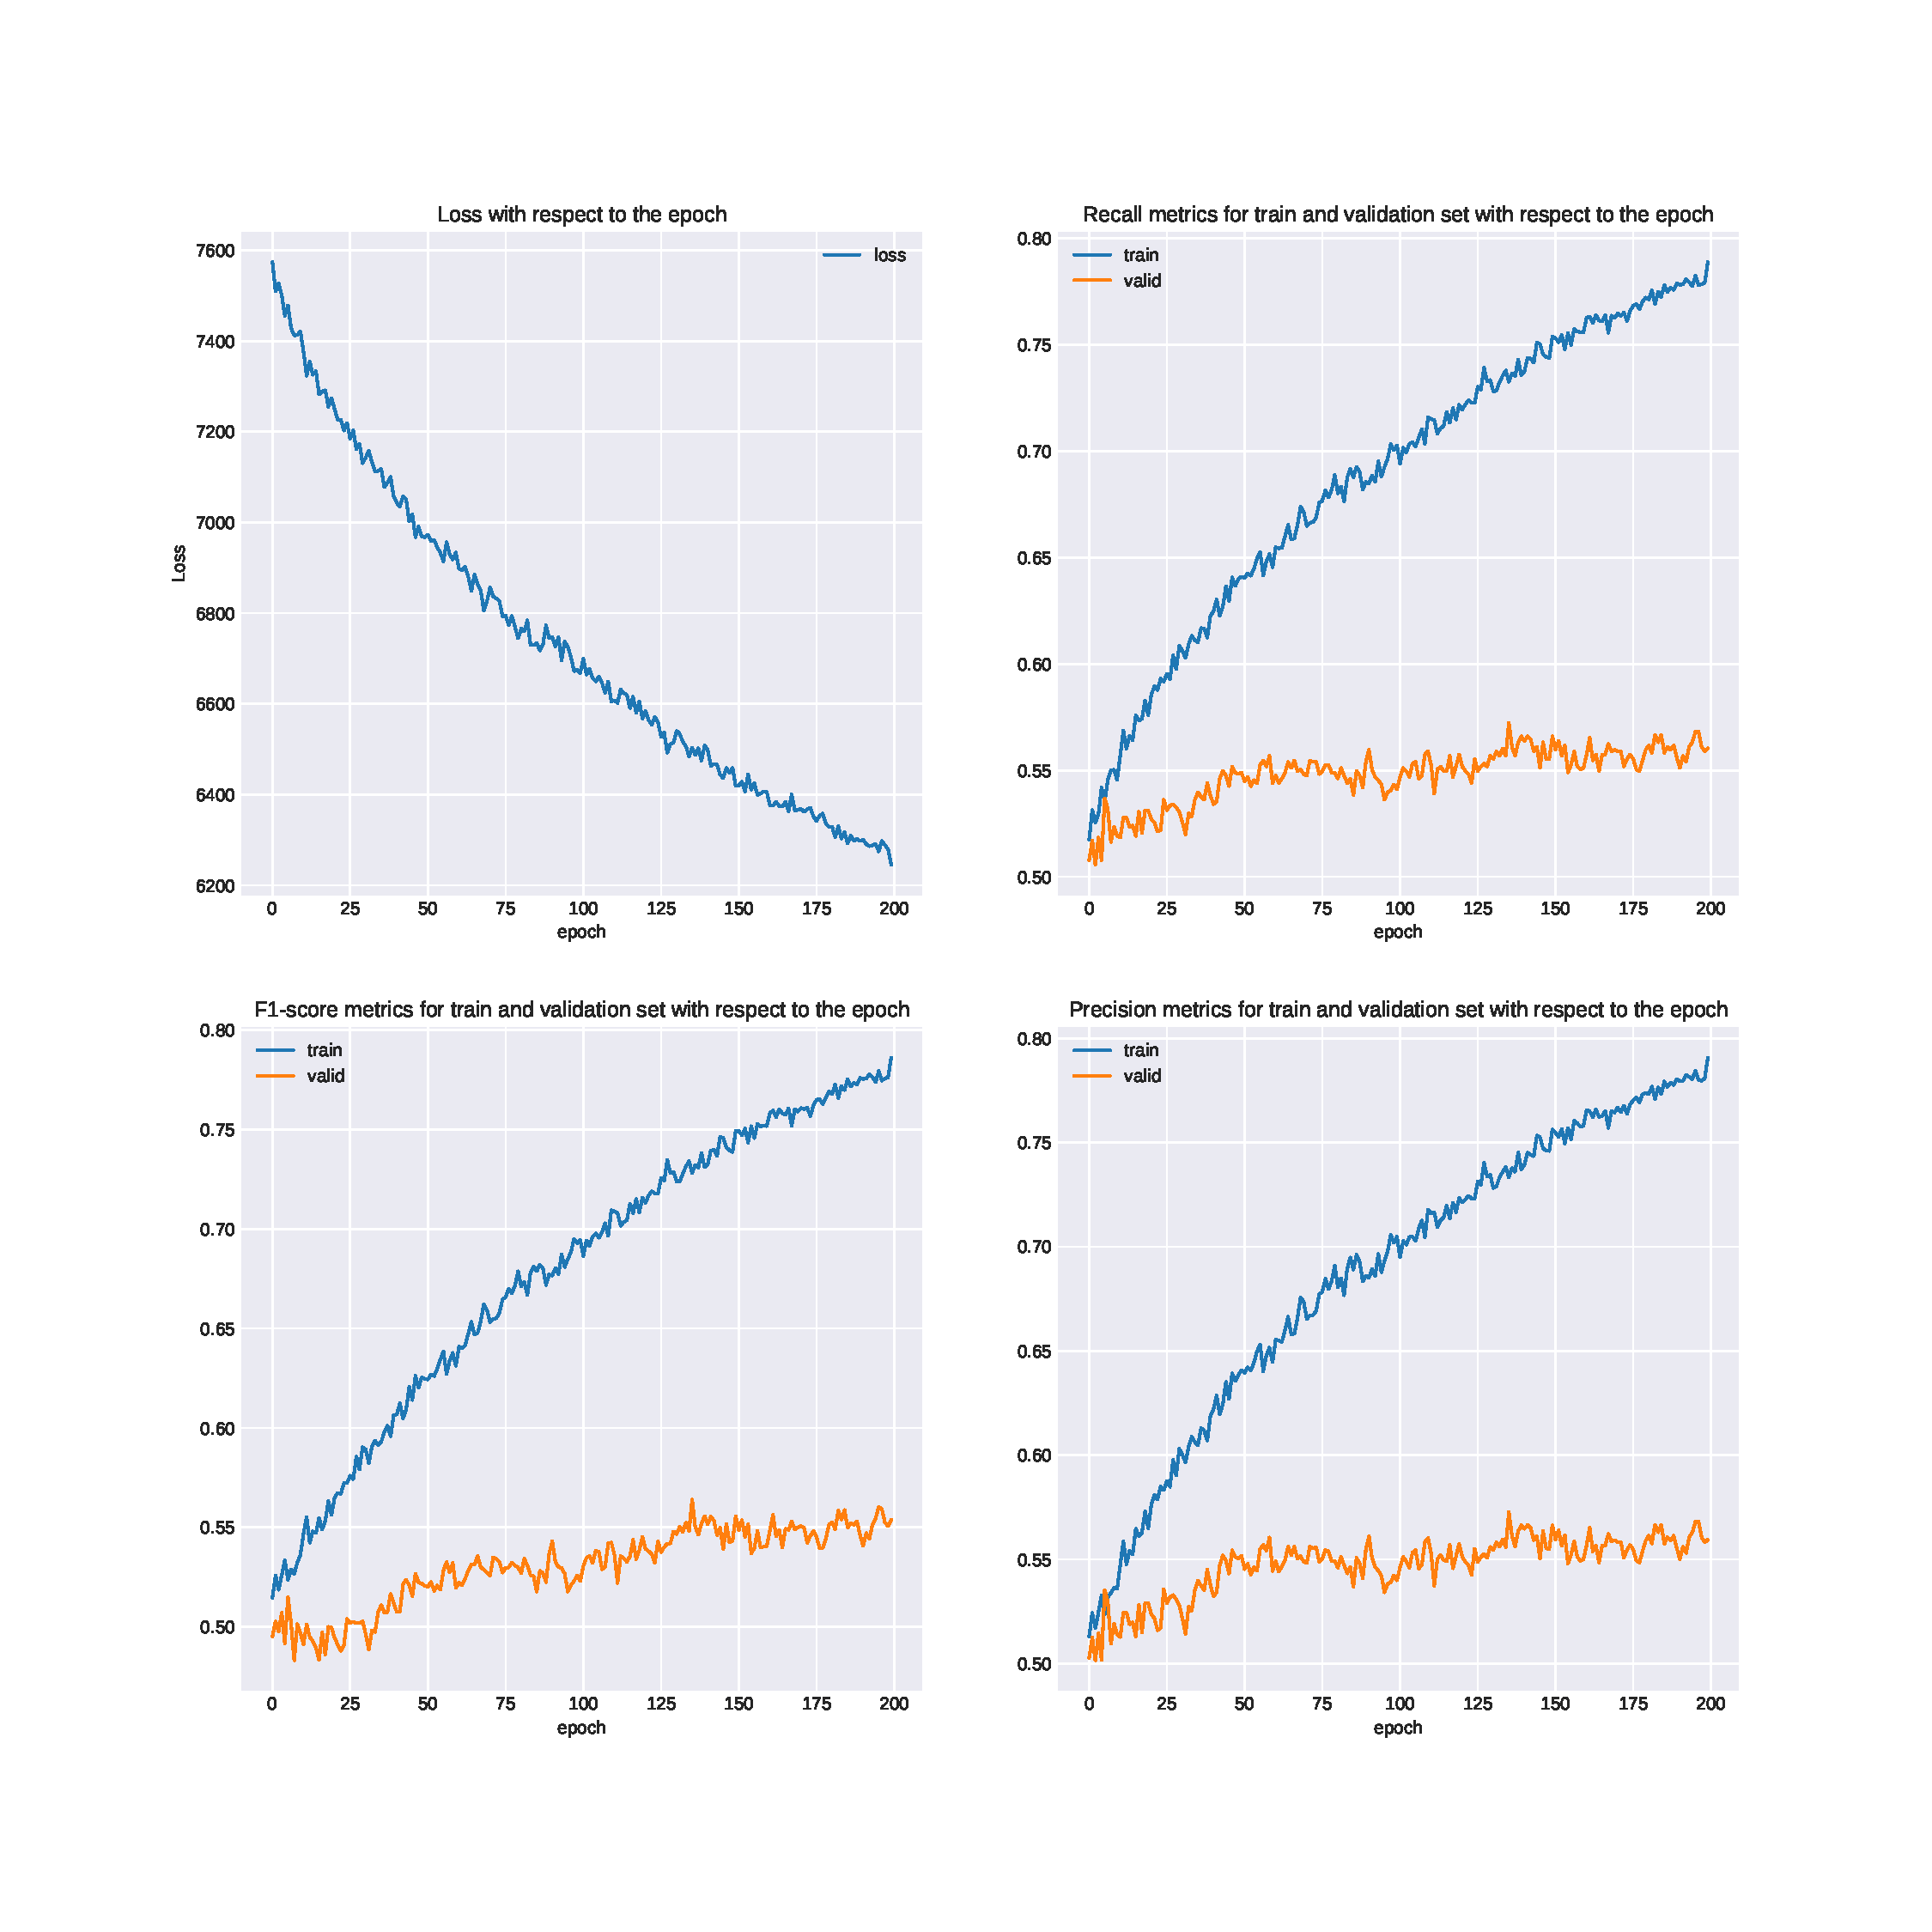
\includegraphics[width=\textwidth]{images/chapitre4/attention-f1}
 \caption{Training and validation of the model with top f1-score}
 \label{fig:chap4:att3:f1}
\end{figure}
Training on 1000 epochs rather than 200 does not improve validation score, but it does for training (\textbf{Figure \ref{fig:chap4:att3:f1.1}}). \\
\begin{figure}
 \centering
 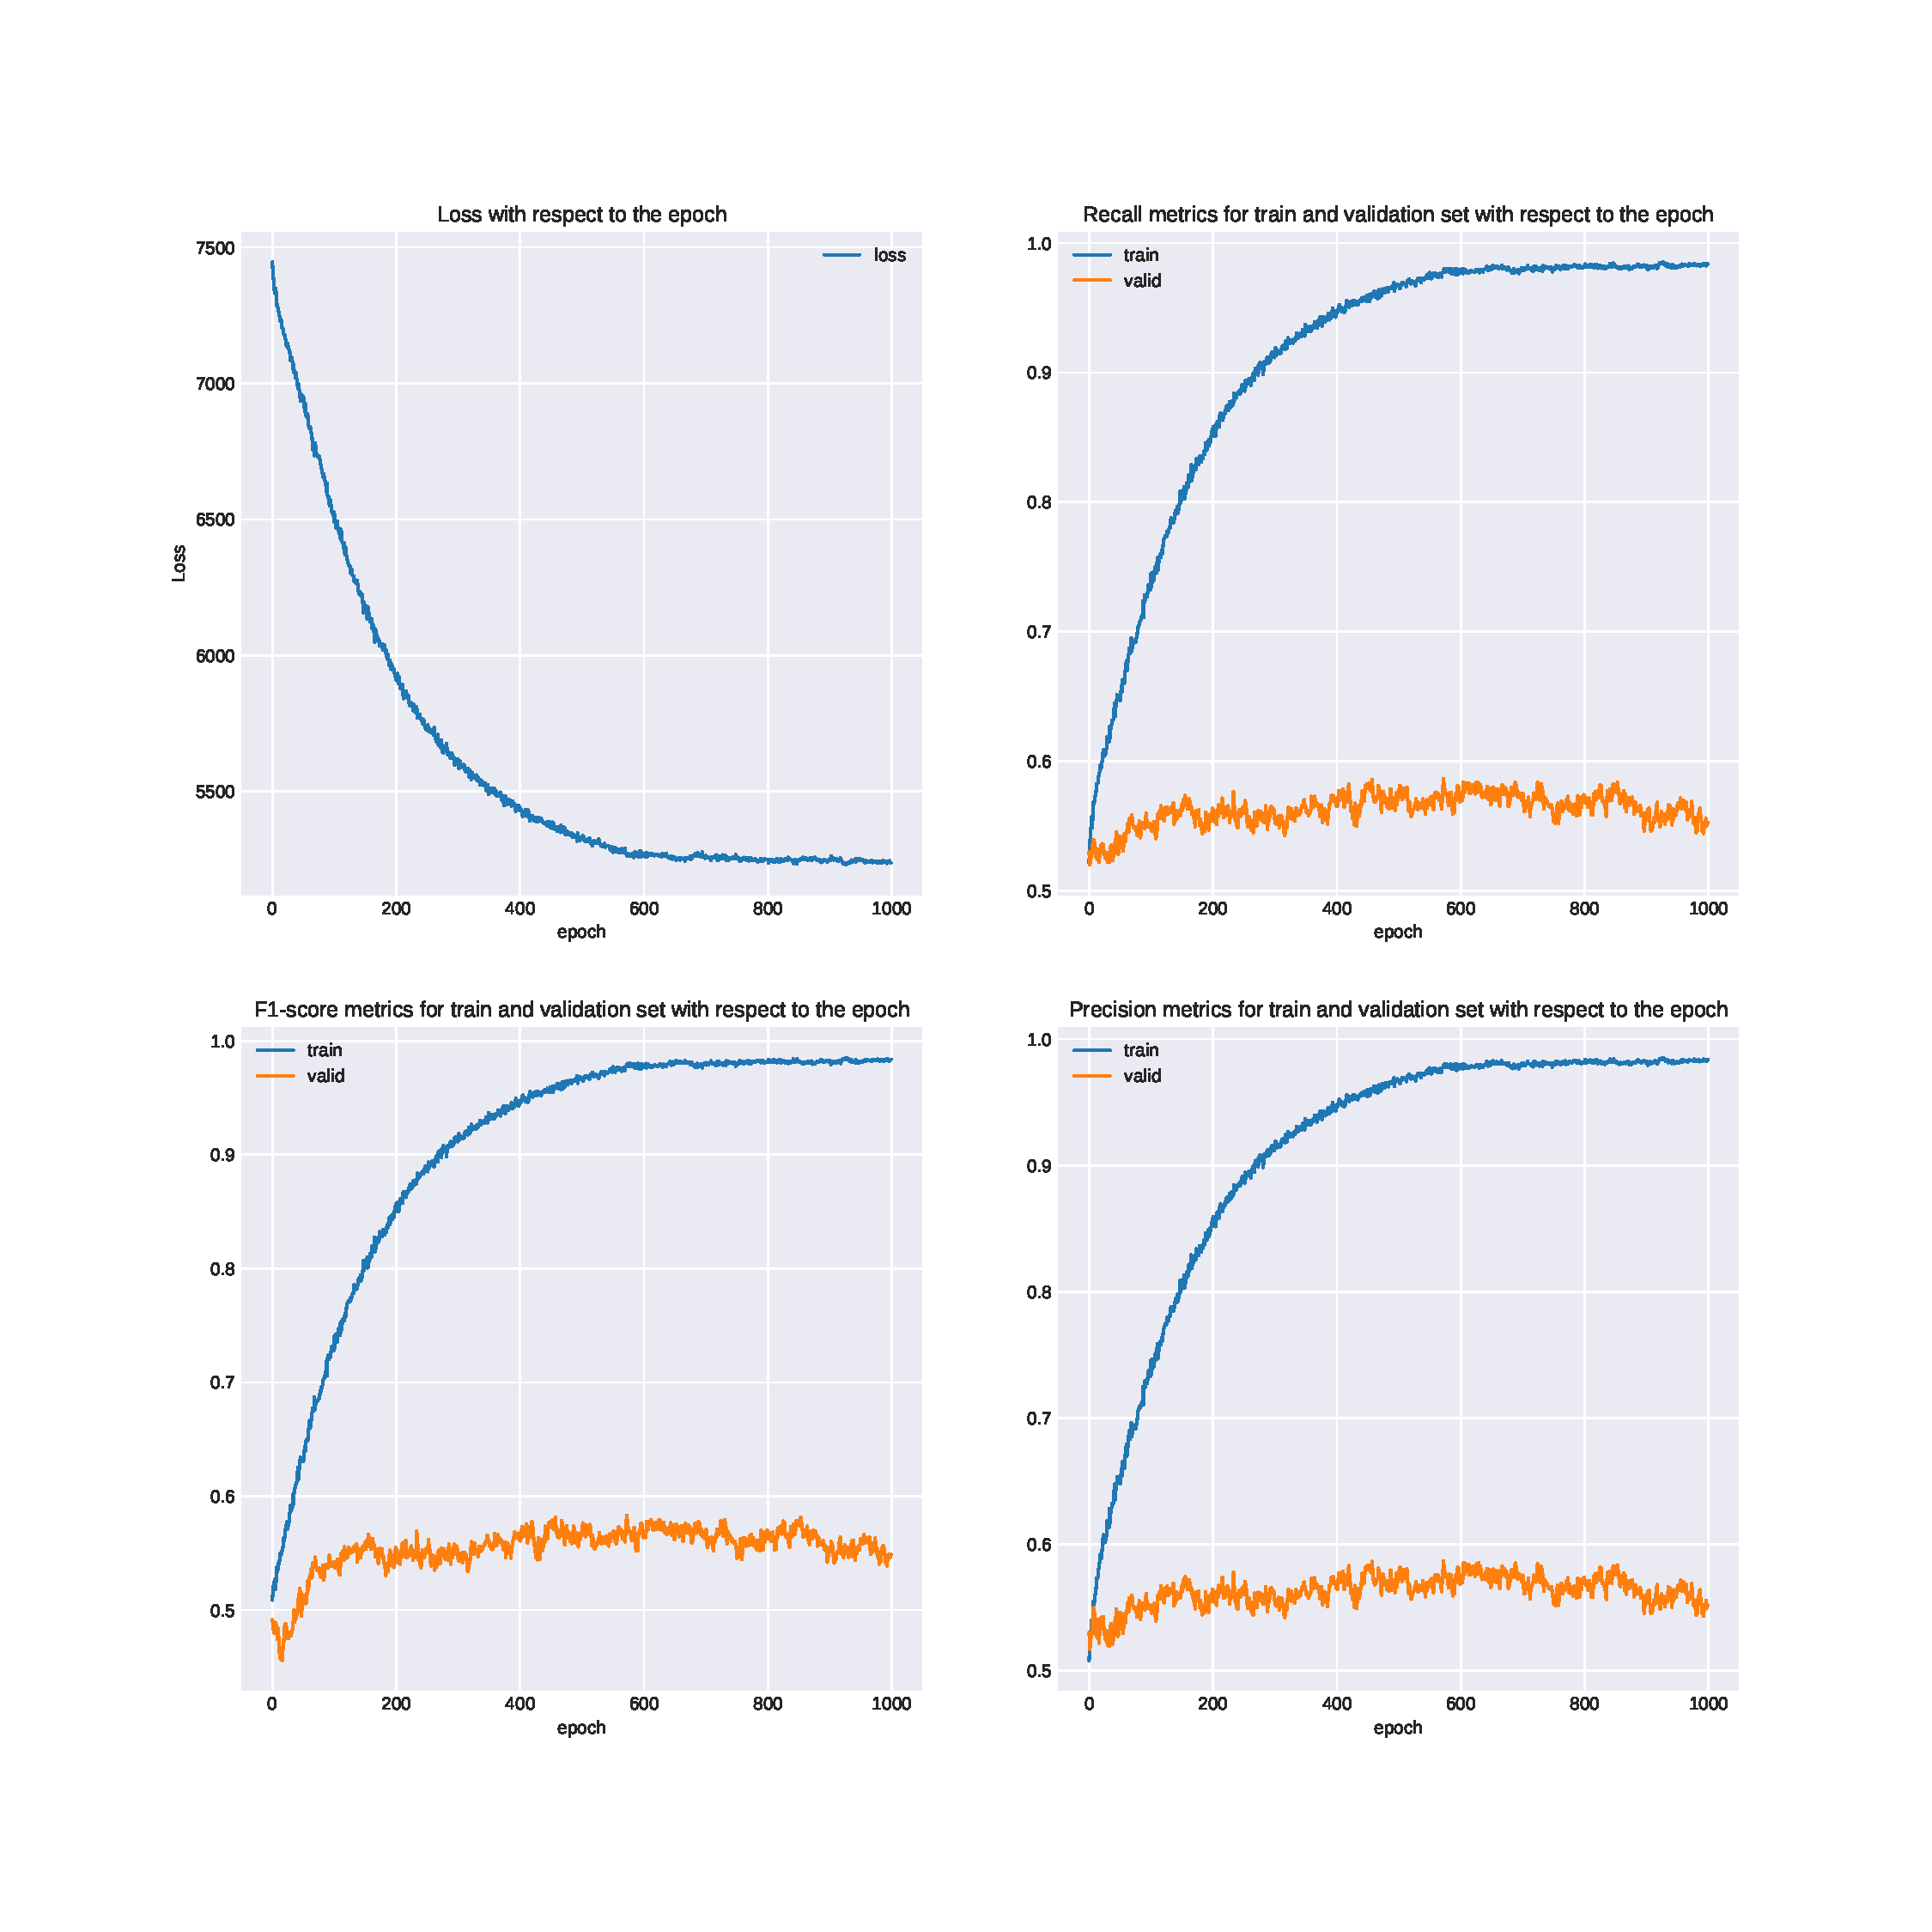
\includegraphics[width=\textwidth]{images/chapitre4/attention3}
 \caption{Training on 1000 epochs rather than 200}
 \label{fig:chap4:att3:f1.1}
\end{figure}
\subsection{Result Analysis}
The previous section shows a few things
\begin{itemize}
 \item LSTMs do not work well,
 \item Adding attention layer improve LSTM results,
 \item Using word2vec rather than training the embedding gives better results.
\end{itemize}
It also shows that despite reaching a very good precision, recall and f1-score on the training set it does not perform well on the validation set. This is a sign of overfitting. In order to avoid this, multiple methods have been applied without showing any improvement. \\

The following methods have been applied: 
\begin{itemize}
 \item Dropout\cite{srivastava2014dropout}, 
 \item batch-normlaziation\cite{Ioffe2015},
 \item reducing network capacity (fewer hidden layers, lower embedding dimensions, less training parameters with word2vec),
 \item Early stopping of training.
\end{itemize}
The highest gain was from using word2vec embedding. This significantly reduces the amount of training parameters, secondly dropout also helped a little. 
\subsection{Testing}
The same way as in \textbf{Chapter \ref{chap3}}, the models will be trained on the parameters that produced the best results on the training set, and trained on training and validation set, and tested on testing set. \\
The parameters used for training are given at \textbf{Table \ref{table:chap4:param}}.
\begin{table}[h]
 \begin{tabular}{|c|ccccc|}
 \hline
 model & embedding size & Sequence Length & num hiddens & dropout & Early Stop\\
 \hline
 LSTM & 300 & 10 & 50 & 0.75 & 126\\
 LSTM + word2vec & 300 & 10 & 50 & 0.0 & 160\\
 Attention & 10 & 20 & 10 & 0.75 & 400\\
 Attention + word2vec & 300 & 20 & 5 & 0.75 & 25\\
 \hline
 \end{tabular}
 \caption{Parameters used for training}
 \label{table:chap4:param}
\end{table}
The results for all four models are given at \textbf{Table \ref{table:chap4:results}}. It shows that the model that works the best is attention network using word2vec embedding, with an accuracy of $61\%$, which is equivalent to ridge classifiers and linear svm. The three other models do not perform well, all having a average precision around $55\%$, which is close to being a random classifier. 
\begin{table}
\centering
\begin{subtable}{\textwidth}
\begin{tabular}{lrrrrr}
\toprule
{} &         fake &     reliable &  accuracy &    macro avg &  weighted avg \\
\midrule
f1-score  &     0.440574 &     0.649551 &  0.569061 &     0.545062 &      0.558340 \\
precision &     0.508274 &     0.599526 &  0.569061 &     0.553900 &      0.559698 \\
recall    &     0.388788 &     0.708683 &  0.569061 &     0.548736 &      0.569061 \\
support   &  1106.000000 &  1428.000000 &  0.569061 &  2534.000000 &   2534.000000 \\
\bottomrule
\end{tabular}
\caption{Simple LSTM}
\end{subtable}
\begin{subtable}{\textwidth}
 \begin{tabular}{lrrrrr}
 \toprule
 {} &         fake &     reliable &  accuracy &    macro avg &  weighted avg \\
 \midrule
 f1-score  &     0.481724 &     0.623040 &  0.563536 &     0.552382 &      0.561361 \\
 precision &     0.500000 &     0.606906 &  0.563536 &     0.553453 &      0.560245 \\
 recall    &     0.464738 &     0.640056 &  0.563536 &     0.552397 &      0.563536 \\
 support   &  1106.000000 &  1428.000000 &  0.563536 &  2534.000000 &   2534.000000 \\
 \bottomrule
 \end{tabular}
 \caption{LSTM + word2vec}
\end{subtable}
\begin{subtable}{\textwidth}
\begin{tabular}{lrrrrr}
\toprule
{} &         fake &     reliable &  accuracy &    macro avg &  weighted avg \\
\midrule
f1-score  &     0.486636 &     0.615597 &  0.560379 &     0.551116 &      0.559310 \\
precision &     0.496241 &     0.606803 &  0.560379 &     0.551522 &      0.558546 \\
recall    &     0.477396 &     0.624650 &  0.560379 &     0.551023 &      0.560379 \\
support   &  1106.000000 &  1428.000000 &  0.560379 &  2534.000000 &   2534.000000 \\
\bottomrule
\end{tabular}
\caption{Attention network}
\end{subtable}
\begin{subtable}{\textwidth}
\begin{tabular}{lrrrrr}
\toprule
{} &         fake &     reliable &  accuracy &    macro avg &  weighted avg \\
\midrule
f1-score  &     0.511397 &     0.676721 &  0.610892 &     0.594059 &      0.604563 \\
precision &     0.565789 &     0.636252 &  0.610892 &     0.601021 &      0.605497 \\
recall    &     0.466546 &     0.722689 &  0.610892 &     0.594618 &      0.610892 \\
support   &  1106.000000 &  1428.000000 &  0.610892 &  2534.000000 &   2534.000000 \\
\bottomrule
\end{tabular}
\caption{Attention Network + word2vec}
\end{subtable}
\caption{Results for the differents models trained with parameters given at \textbf{Table \ref{table:chap4:param}}.}
\label{table:chap4:results}
\end{table}
\section{Attention Mechanism on fake news corpus}
\subsection{Model Selection}
The two models using word2vec embedding have shown to work better than their counterparts, this why only these two methods will be tested on \textbf{Fake News Corpus} for comparison as very good results have already been obtained. \\

It shows out that in this case LSTMs works better than Attention Mechanism, but as in previous section does not reach machine learning results. \\

The best LSTM obtained use sequence of 200 words and 200 hidden layers, with an average precision of $0.929376$ on the validation set. The training plots of this particular model are shown at \textbf{Figure \ref{chap4:fig:lstm5.1}}.\\
\begin{figure*}
 \centering
 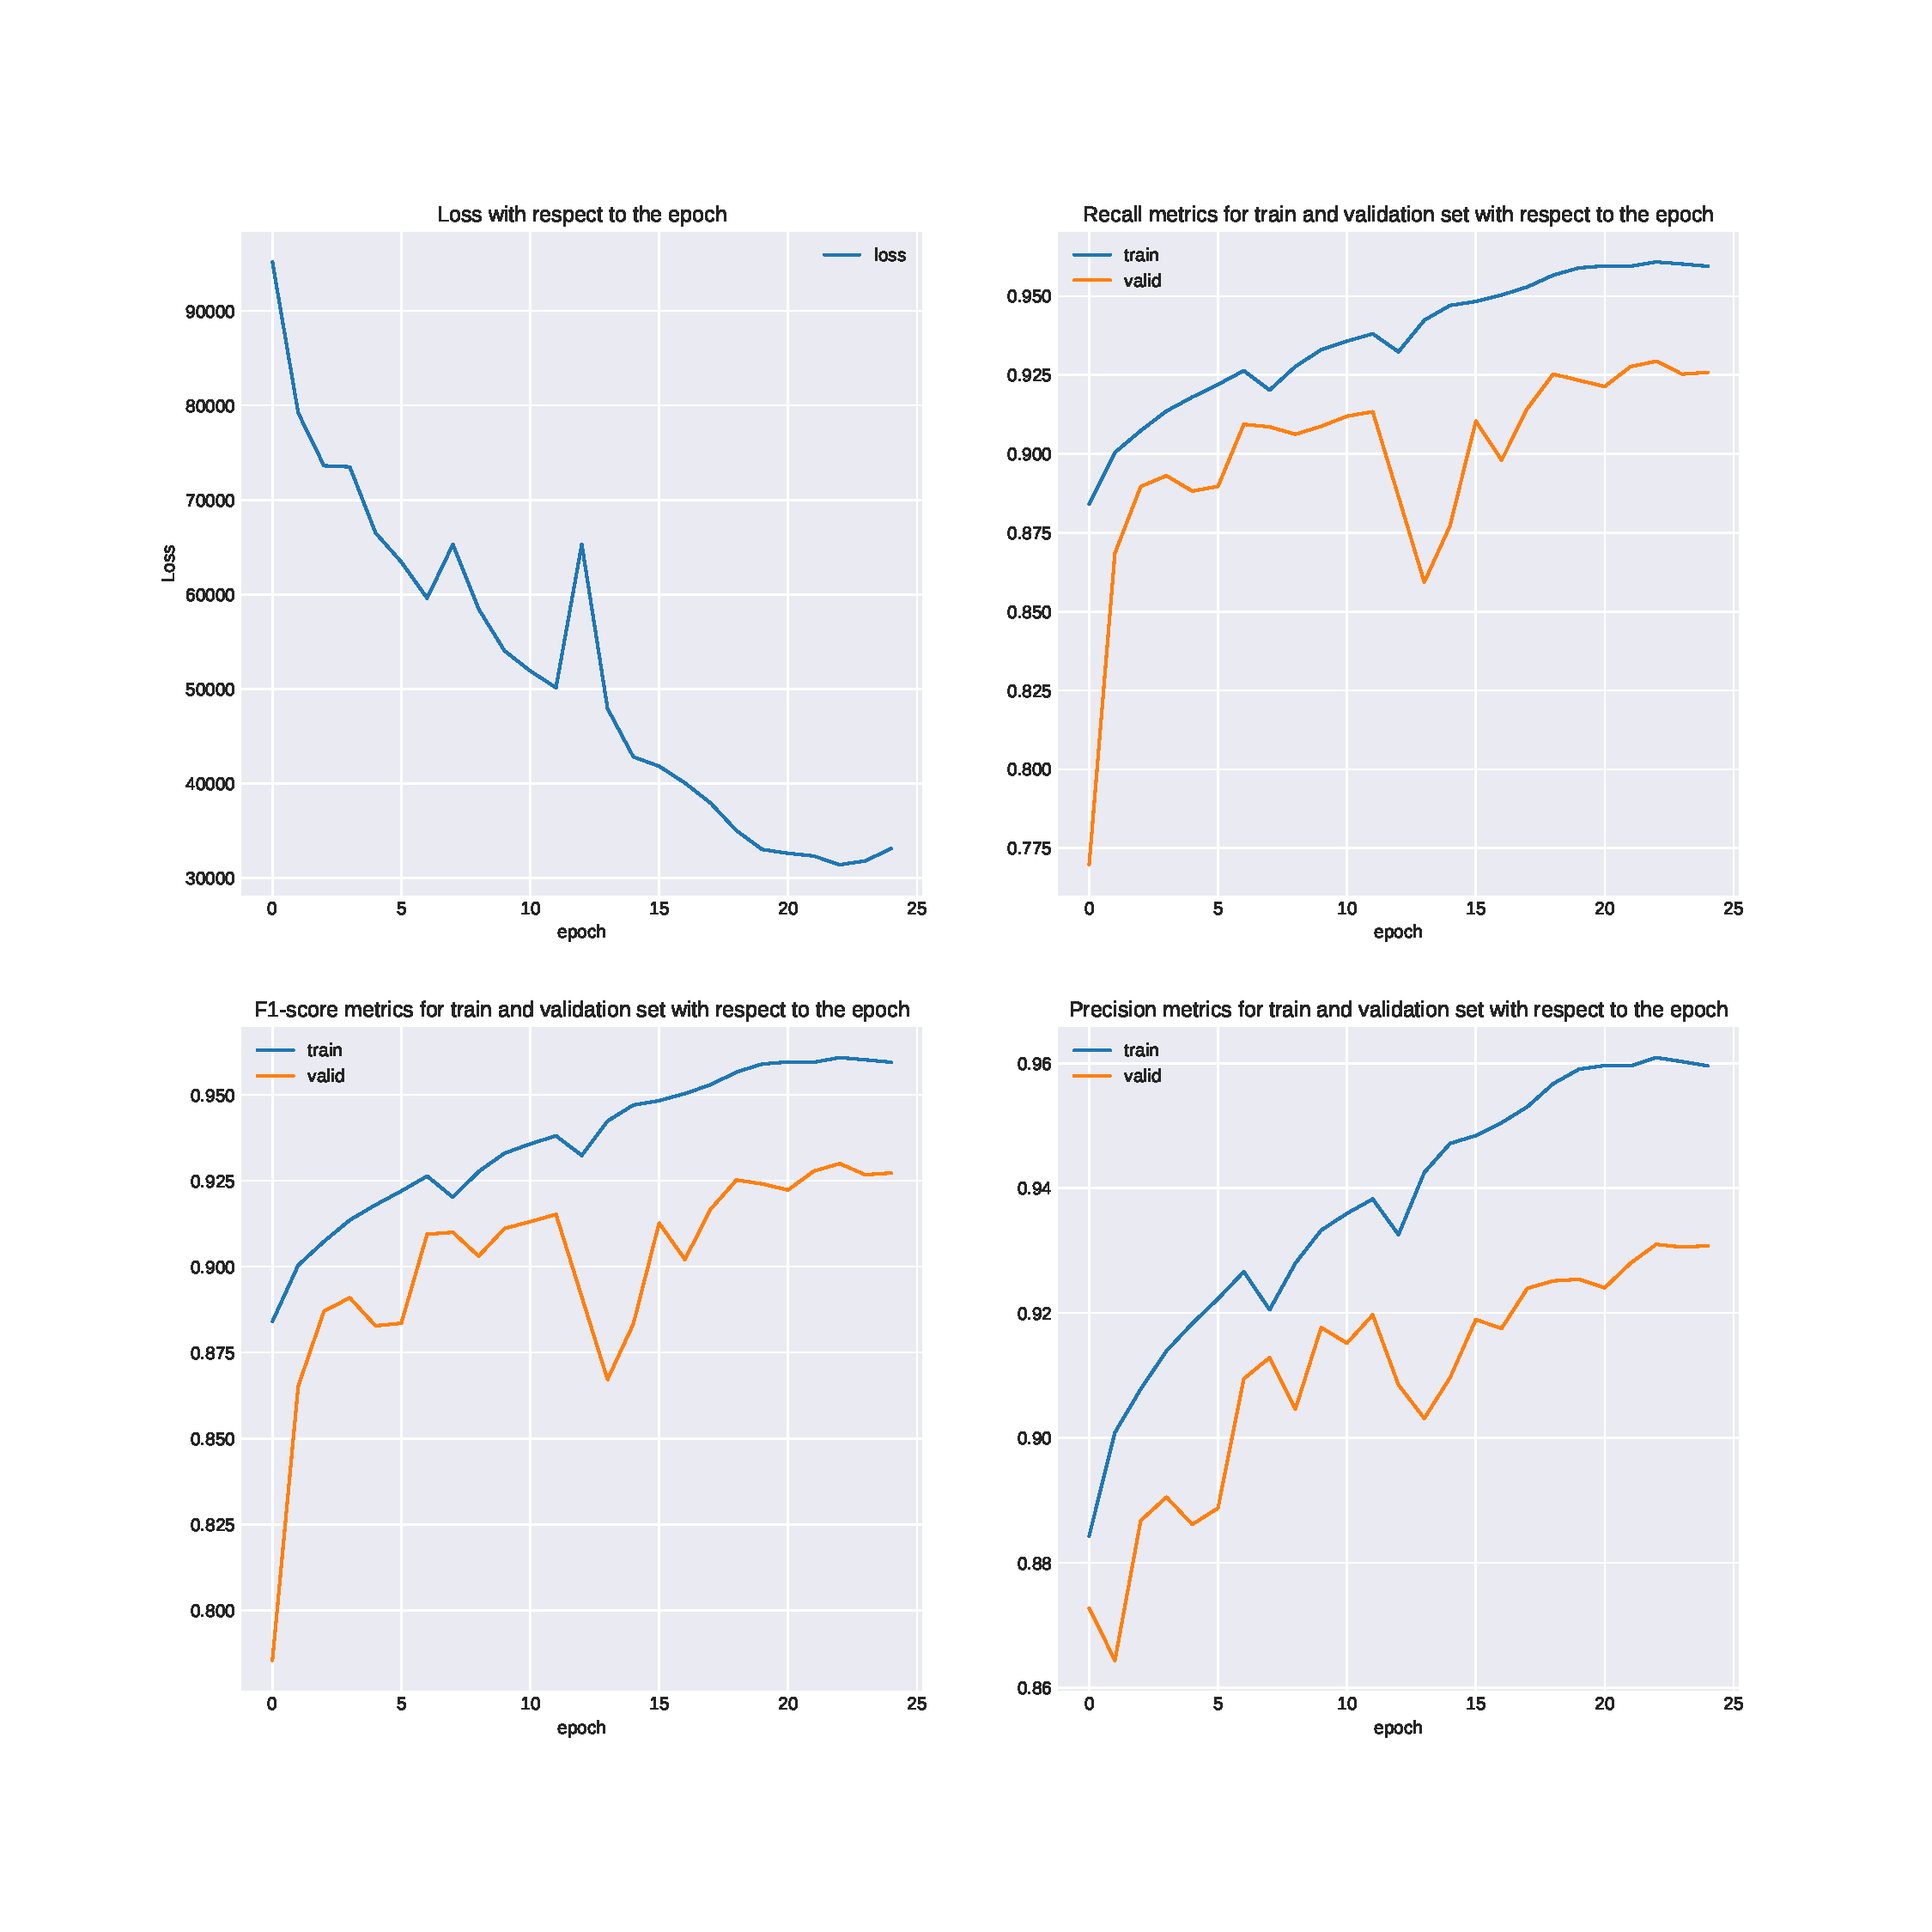
\includegraphics[width=\textwidth]{images/chapitre4/lstm5}
 \caption{Training plots of the best LSTM using word2vec embedding.}
 \label{chap4:fig:lstm5.1}
\end{figure*} 

In the case of attention mechanism, training on the \textbf{Fake News Corpus} has shown to be harder than on the \textbf{Liar-Liar Corpus} as using too large learning rate would lead to oscillating loss and too small learning rate lead to halting the loss decrease. This can be seen at \textbf{Appendix \ref{appendix2:training_plot2}}. \\

The same parameters as for the LSTM will be used for training the Attention Network. Its training plot is available at \textbf{Figure \ref{chap4:fig:attention5}}.
\begin{figure*}
 \centering
 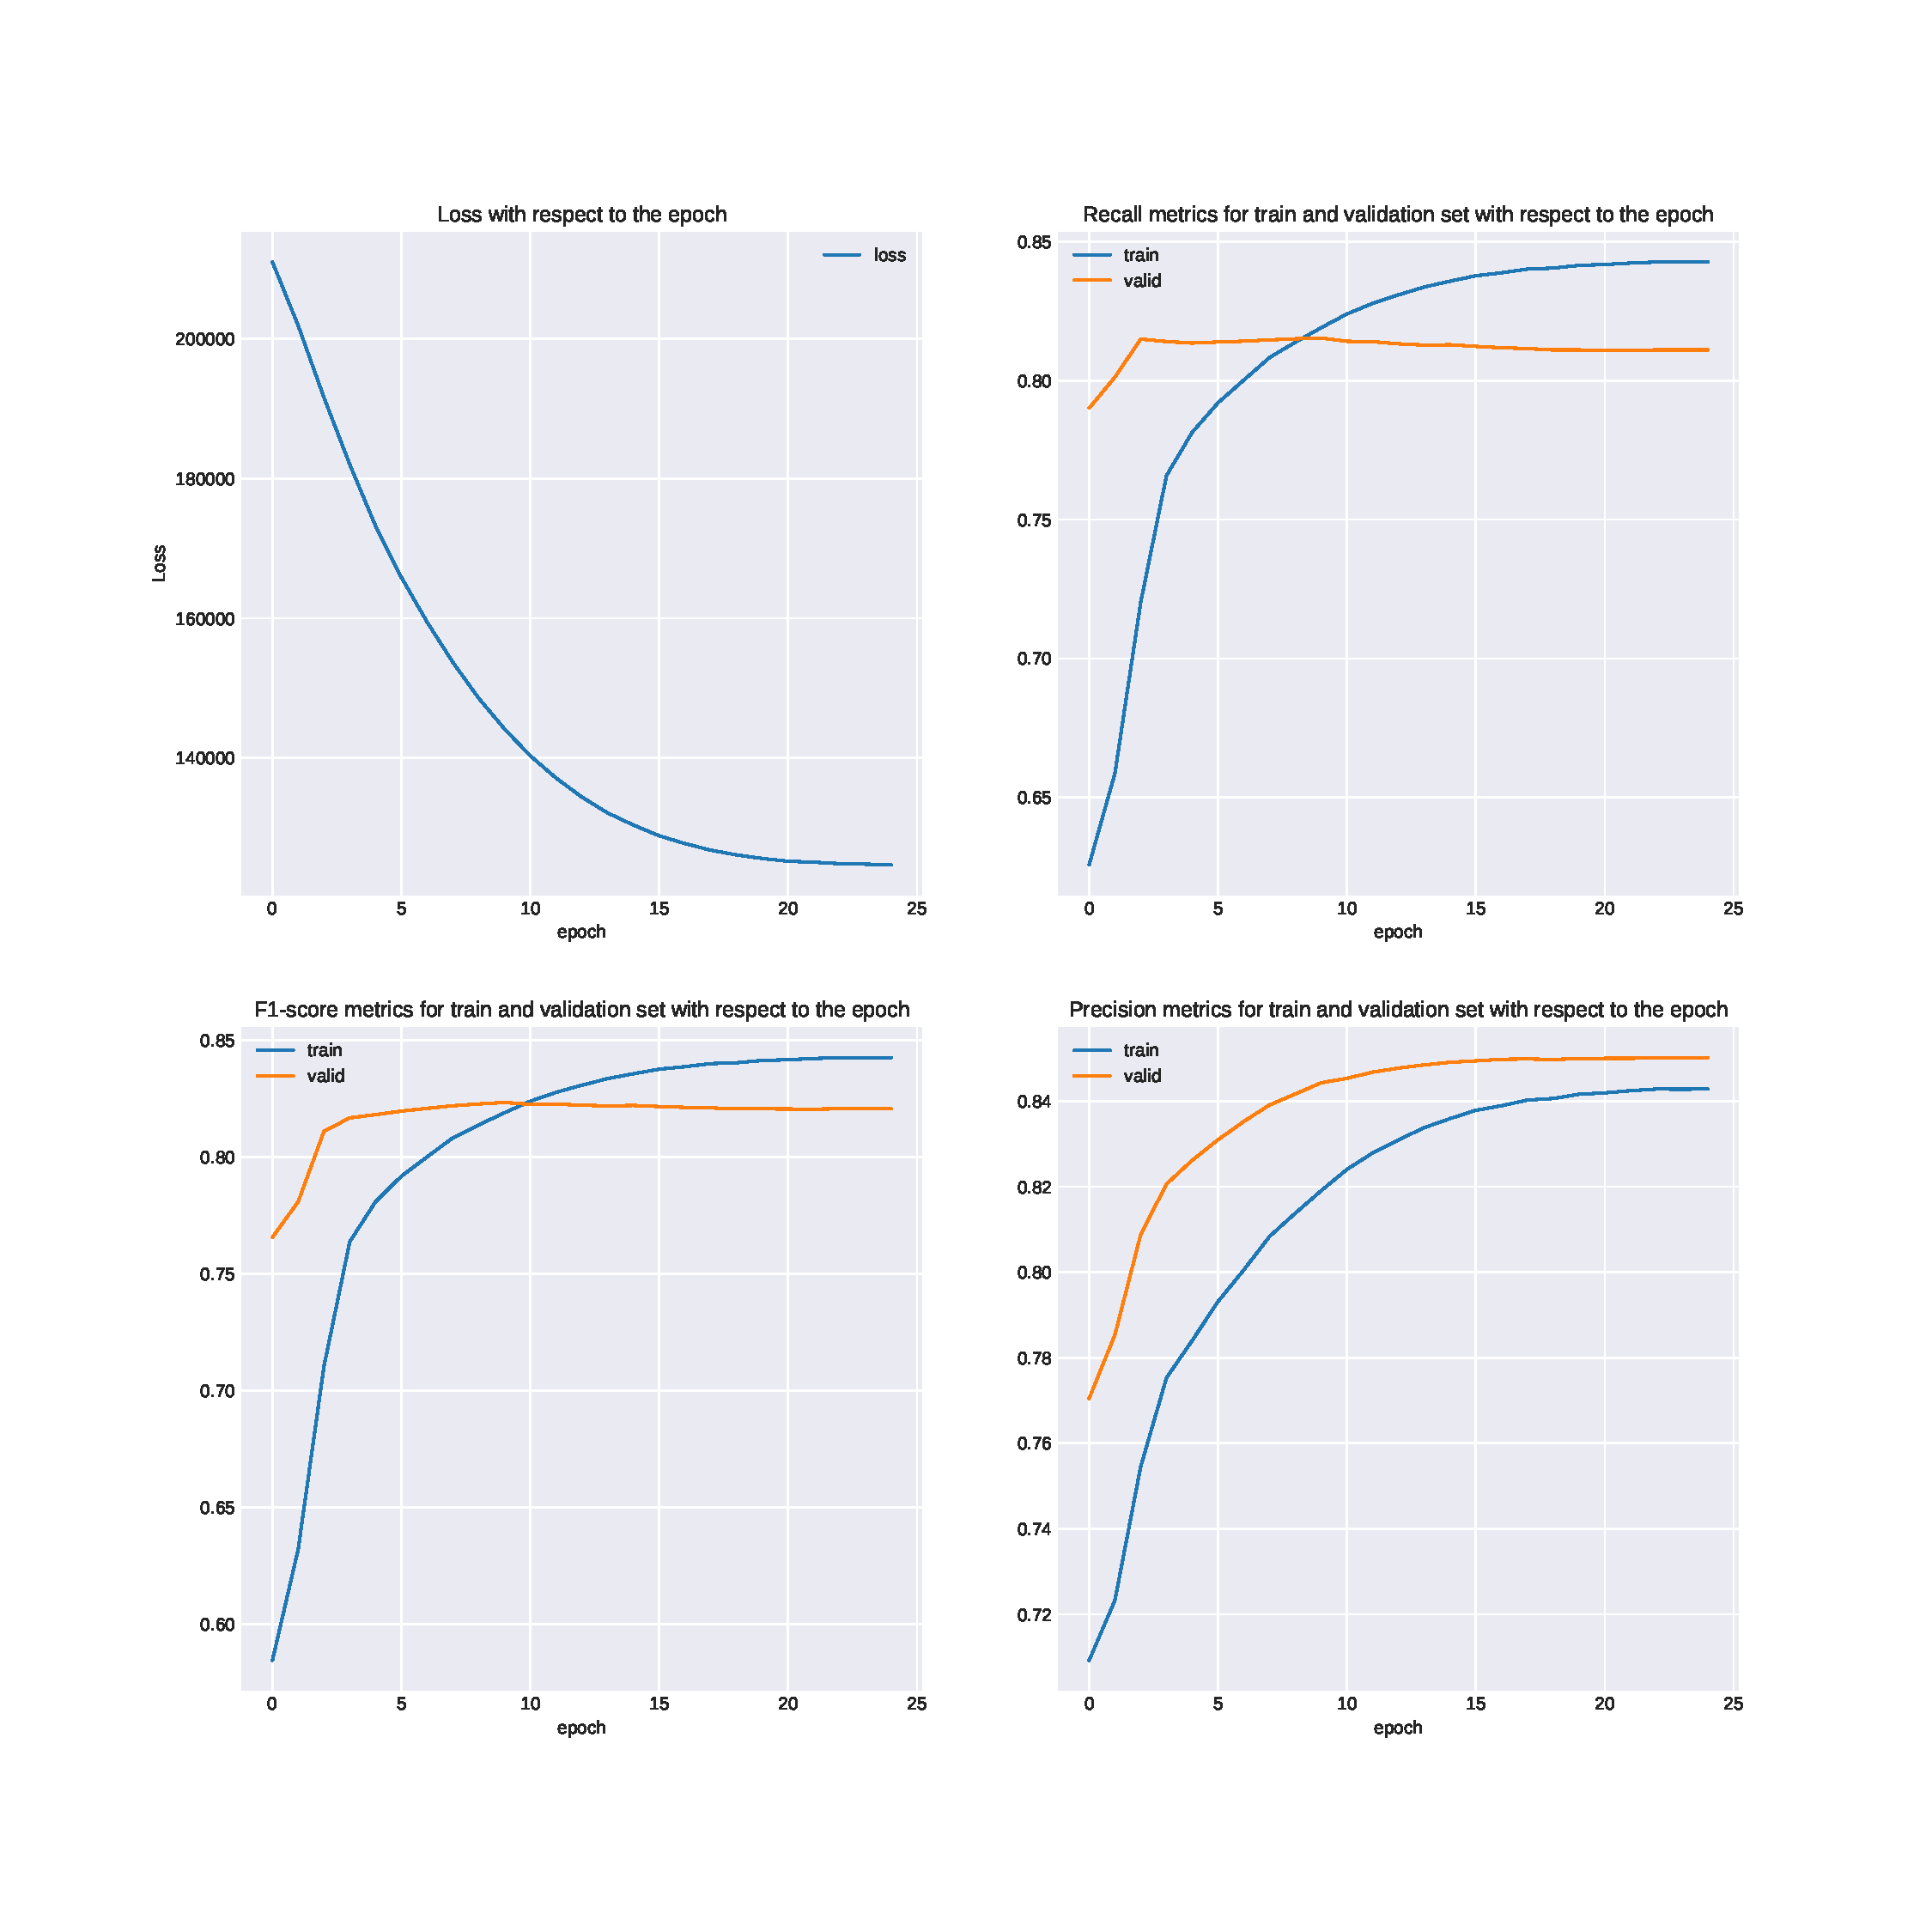
\includegraphics[width=\textwidth]{images/chapitre4/attention5}
 \caption{Training plots of the best attention network using word2vec embedding.}
 \label{chap4:fig:attention5}
\end{figure*} 
The final results are given at \textbf{Table \ref{table:chap4:results2}}. It shows that for the same parameters LSTM works better than Attention Network on this particular dataset. It shows that LSTM place below Linear SVM and Ridge Classifier and above Decision Tree and Na\"{i}ve-Bayes in terms of accuracy. 
\begin{table}
 \begin{subtable}{\textwidth}
  \begin{tabular}{lrrrrr}
  \toprule
  {} &          fake &      reliable &  accuracy &     macro avg &  weighted avg \\
  \midrule
  f1-score  &      0.856568 &      0.947577 &  0.923217 &      0.902073 &      0.924724 \\
  precision &      0.806655 &      0.969503 &  0.923217 &      0.888079 &      0.928611 \\
  recall    &      0.913066 &      0.926621 &  0.923217 &      0.919843 &      0.923217 \\
  support   &  17496.000000 &  52181.000000 &  0.923217 &  69677.000000 &  69677.000000 \\
  \bottomrule
  \end{tabular}
  \caption{LSTM + word2vec results on \textbf{Fake News Corpus}}
 \end{subtable}
 \begin{subtable}{\textwidth}
  \begin{tabular}{lrrrrr}
  \toprule
  {} &      reliable &          fake &  accuracy &     macro avg &  weighted avg \\
  \midrule
  f1-score  &      0.850296 &      0.687493 &  0.797566 &      0.768894 &      0.809416 \\
  precision &      0.952876 &      0.561344 &  0.797566 &      0.757110 &      0.854562 \\
  recall    &      0.767655 &      0.886774 &  0.797566 &      0.827215 &      0.797566 \\
  support   &  52181.000000 &  17496.000000 &  0.797566 &  69677.000000 &  69677.000000 \\
  \bottomrule
  \end{tabular}
  \caption{Attention Network + word2vec on \textbf{Fake News Corpus}}
 \end{subtable}
 \caption{Final result on testing set for LSTM and attention network using word2vec.}
 \label{table:chap4:results2}
\end{table}
It is likely to be possible to reach results as well as LSTM or even better for the Attention Network, but due to technical and time constraints I was not able to experiment further. For instance, using longer sequence length and more hidden units with a smaller learning rate might have overcome this problem. 
\section{Conclusion}
In this chapter I have investigated how state-of-the-art deep learning models work on fake news detection, and it shows that for the particular case of fake news detection it does not outperform traditional machine learning methods. I have also made some addition to the original model that improves the performances by a few percent by replacing the tunable word embedding by constant one using word2vec. It shows out that it helps reduce overfitting and increase result on the testing set. \\

A hypothesis to explain why these two deep learning methods do not works as well as machine learning methods is the fact that in this case text are required to be the same size. Which means that some of them require some padding and the other are srunk. In the second case, information is lost. \\

In addition, it shows that \textbf{Liar-Liar Corpus} is hard to work on, with $60\%$ precision, when \textbf{Fake News Corpus} still have good results. 